\chapter{Novel PPL inference techniques}
\label{chap:infEngines}

In the previous chapter we attempted to re-write probabilistic programs in such a way as to improve the performance of local, single-site, Metropolis-Hastings inference. However this appraoch may prove too limiting, and it's natural to also explore different inference techniques that may perform better at least on some subset of possible models. In this chapter we explore one such technique, slice sampling, while also briefly looking at some issues of tangential interest.

\section{Preliminaries}
In order to implement a PPL based on a new inference technique we need to understand both how the inference technique in question works and how we may build a PPL in general.

\subsection{Slice sampling}
\todo{add basic description of slice sampling}

\subsection{Basic PPL Construction}
\todo{add basic description of lightweight style PPL construction}

\section{Stochastic Python}
\todo{add description of implementation, space permitting}

\section{Slice sampling inference engine}
\subsection{Custom Slice Sampling and Metropolis on Tdf models}

As a preliminary test, we implement custom slice sampling and local metropolis-hastings algorithms for the Tdf continuous and Tdf21 continuous models. 

Comparison of time to neighbourhood of mode between this algorithm and naive metropolis, on the 2 tdf datasets, is presented in Figure \ref{fig:SliceMetCustPerf}

\begin{figure}[H]
    \centering
    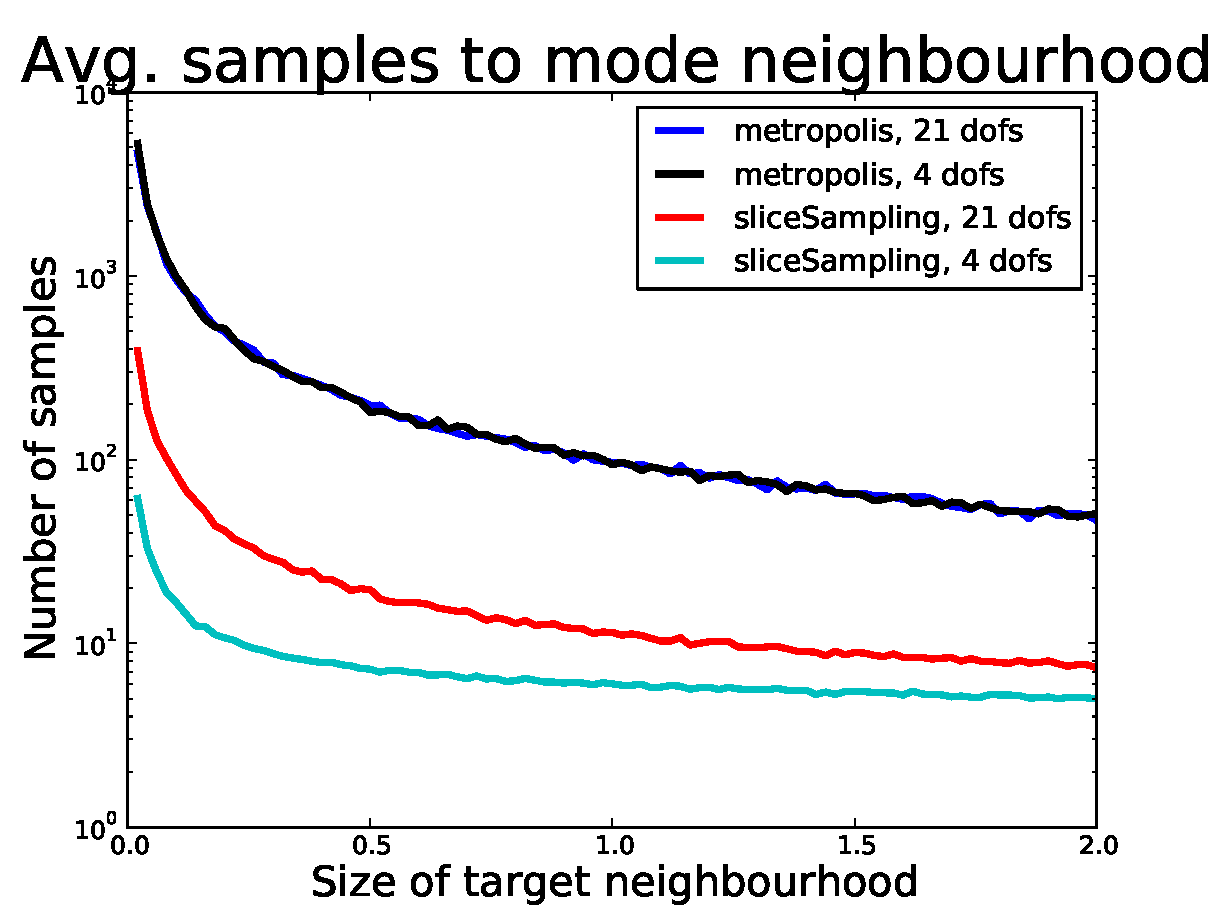
\includegraphics[width=0.8\textwidth]{SliceMetCustPerf}
    \caption{Burn-in time for local metropolis-hastings and slice sampling, on the two continuous Tdf models, as the target neighbourhood varies.}
    \label{fig:SliceMetCustPerf}
\end{figure}

Slice sampling seems to do significantly better (in fact better than any of the partitioned priors did averaged over the all mode placements)
However the performance of slice sampling does seem to vary with the shape of the likelihood distribution. To investigate this we can assume the likelihood is a Gaussian and see how the performance changes as we vary its properties.

\begin{figure}[H]
    \centering
    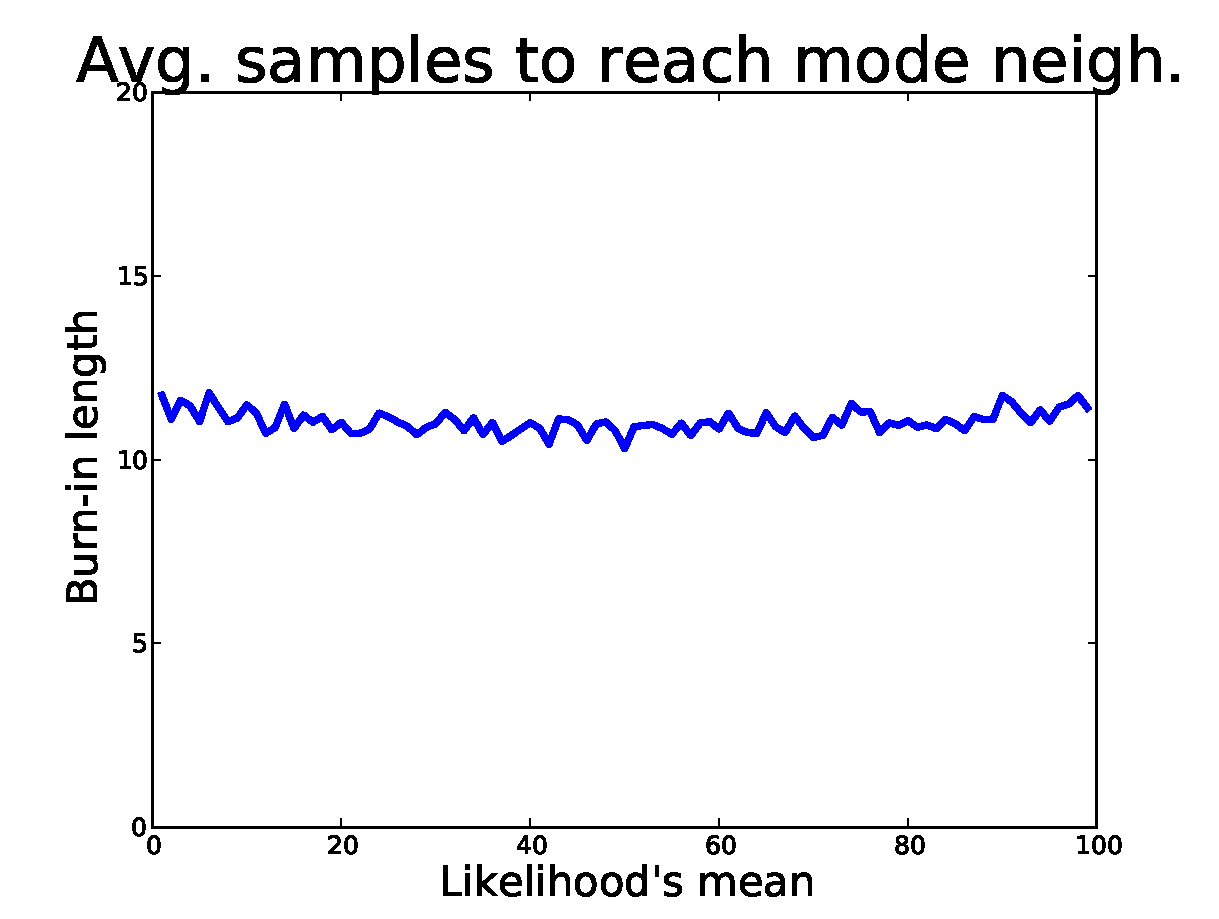
\includegraphics[width=0.8\textwidth]{SliceSampsMean}
    \caption{Burn-in time for slice samplin, when assuming an underlying Gaussian likelihood function which's mean we vary.}
    \label{fig:SliceSampsMean}
\end{figure}

\begin{figure}[H]
    \centering
    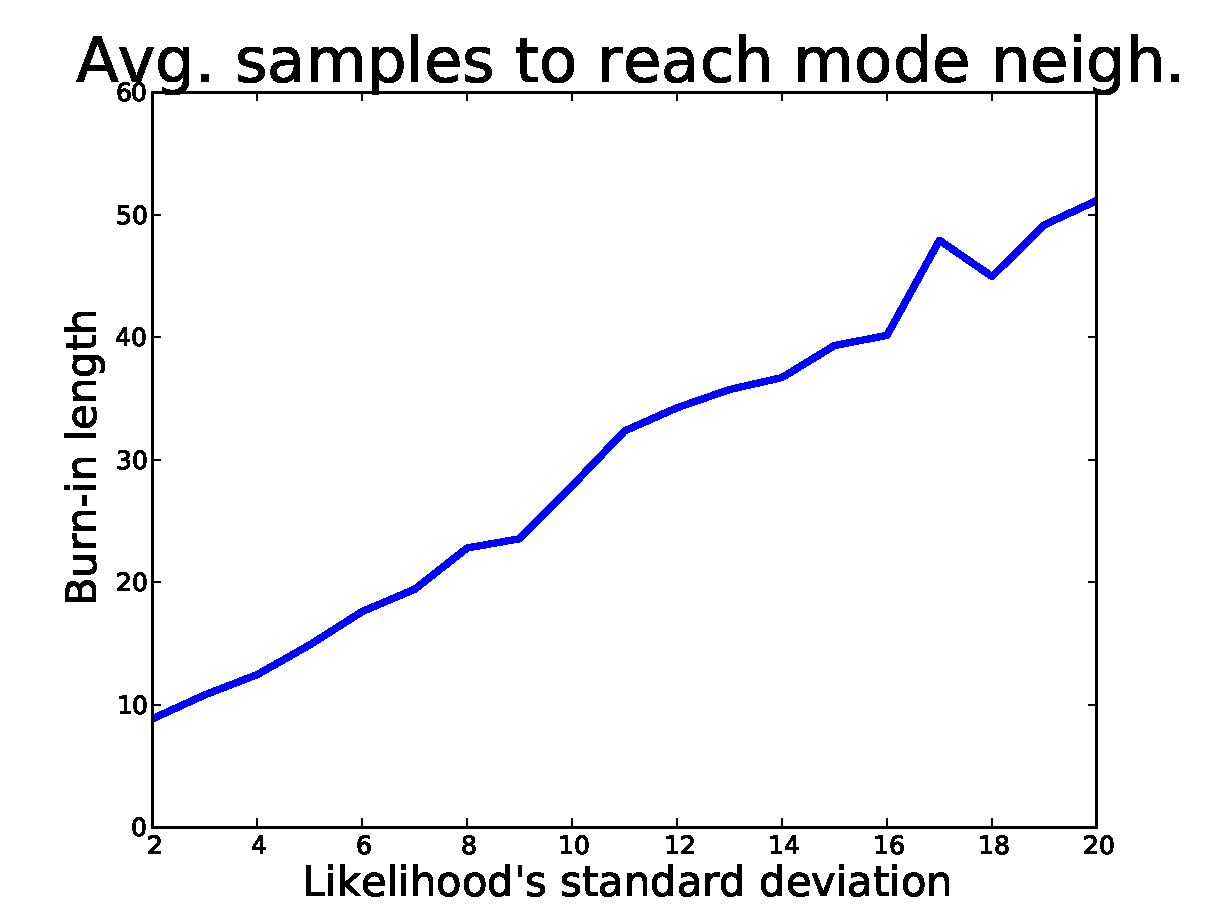
\includegraphics[width=0.8\textwidth]{SliceSampsStd}
    \caption{Burn-in time for slice samplin, when assuming an underlying Gaussian likelihood function which's standard deviation we vary.}
    \label{fig:SliceSampsStd}
\end{figure}

It seems that the placement of the likelihood in the interval doesn't matter, but the width of the distribution does. For reference, the minimum and maximum standard deviations tested conform to the Gaussians in Figures \ref{fig} and \ref{fig}.

\begin{figure}[H]
    \centering
    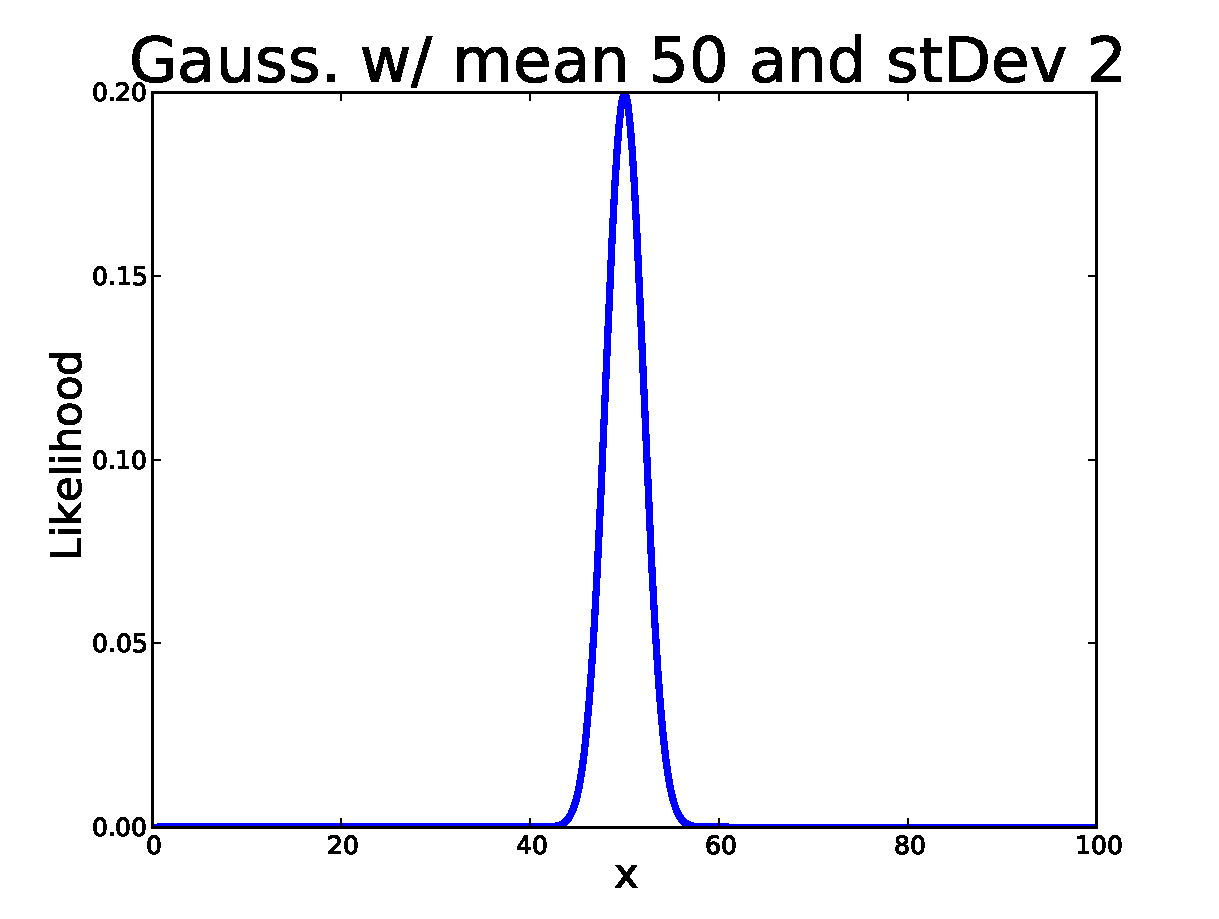
\includegraphics[width=0.8\textwidth]{Gauss2}
    \caption{The smallest Gaussian standard deviation considered in the experiment from Figure \ref{fig}}
    \label{fig:Gauss2}
\end{figure}

\begin{figure}[H]
    \centering
    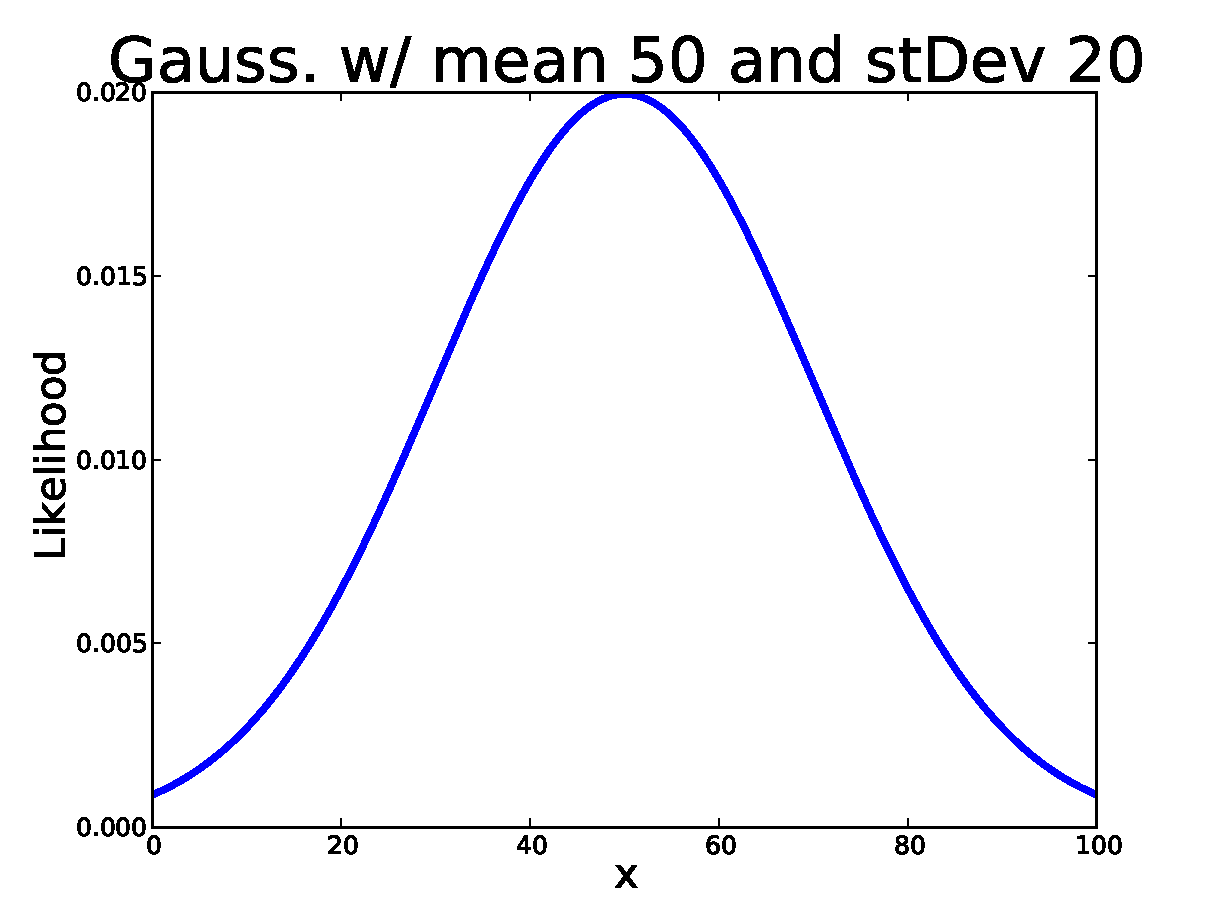
\includegraphics[width=0.8\textwidth]{Gauss20}
    \caption{The largest Gaussian standard deviation considered in the experiment from Figure \ref{fig}}
    \label{fig:Gauss20}
\end{figure}

Next we look at the mixing properties of local metropolis-hastings and slice sampling. To test these we repeat the experiments performed in Chapter \ref{chap} by looking at the sample evolution, the sample autocorellation and the empirical distributions obtained by the two methods.
For the comparison to be fair we keep the number of log-likelihood computations performed by the two methods equal. This means that, while metropolis-hastings is allowed 10,000 samples, we only take 1962 from slice sampling (since, on this model, slice sampling averages just over 5 likelihood computations per extracted sample).

\begin{figure}[H]
    \centering
    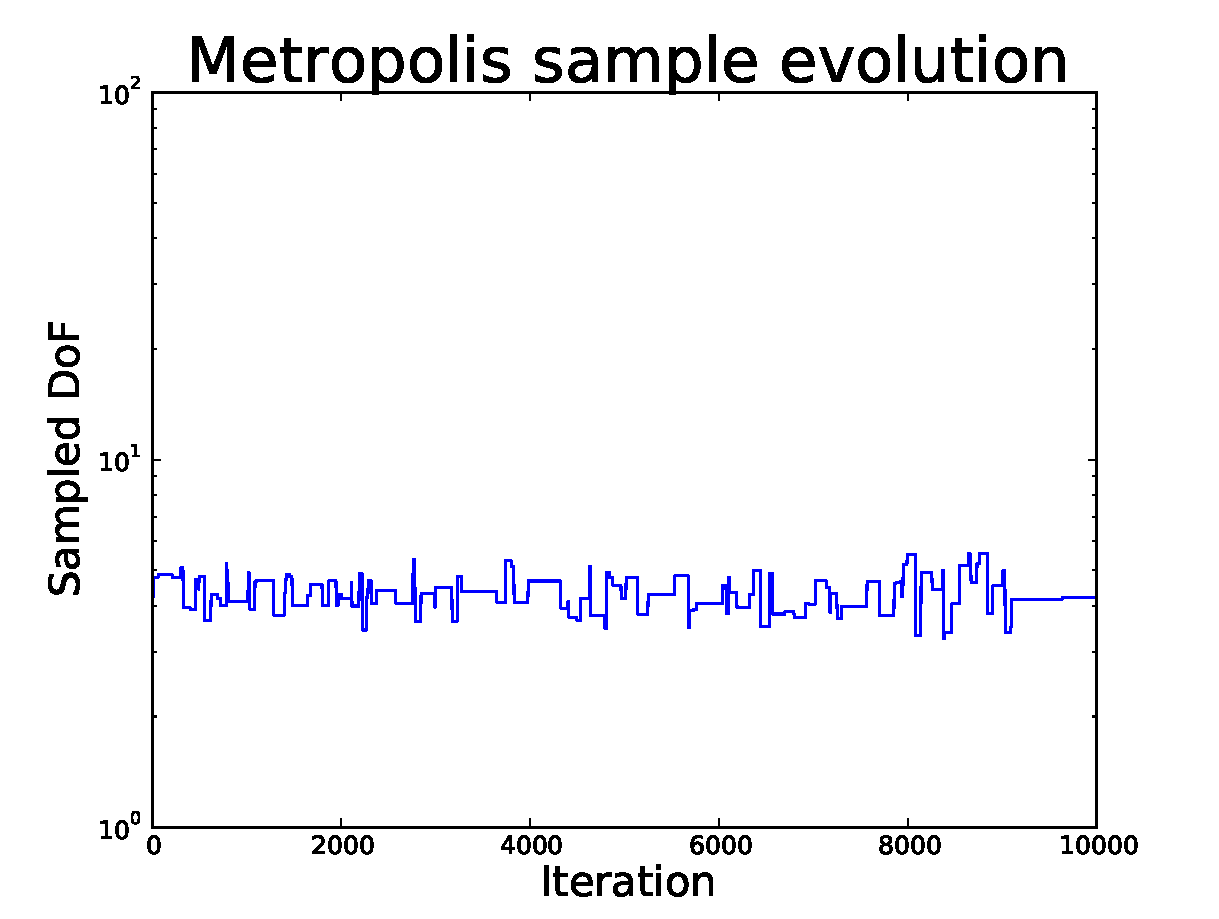
\includegraphics[width=0.8\textwidth]{MetSampEvol}
    \caption{Sample evolution of the metropolis-hastings algorithm on the Tdf continuous model}
    \label{fig:MetSampEvol}
\end{figure}

\begin{figure}[H]
    \centering
    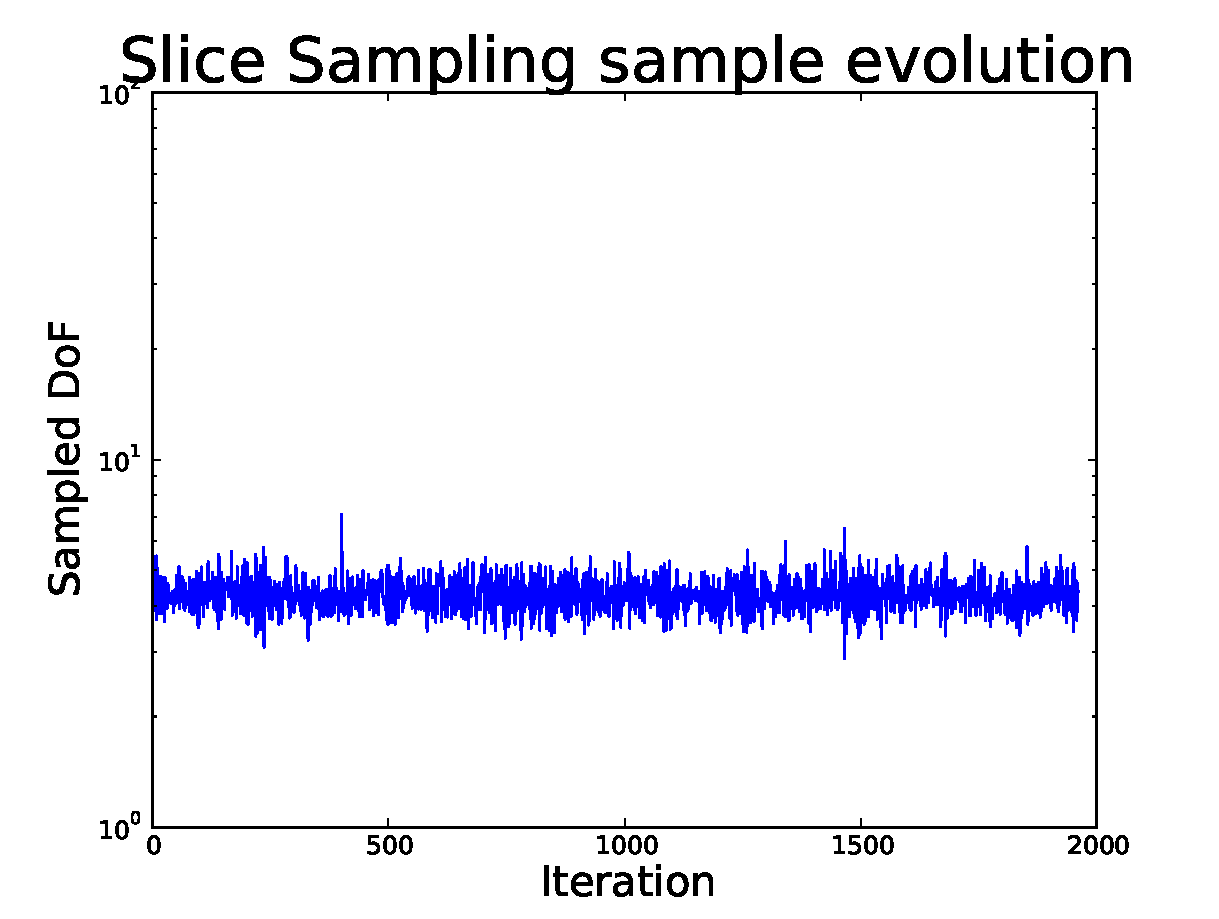
\includegraphics[width=0.8\textwidth]{SliceSampEvol}
    \caption{Sample evolution of the slice sampling algorithm on the Tdf continuous model}
    \label{fig:SliceSampEvol}
\end{figure}

\begin{figure}[H]
    \centering
    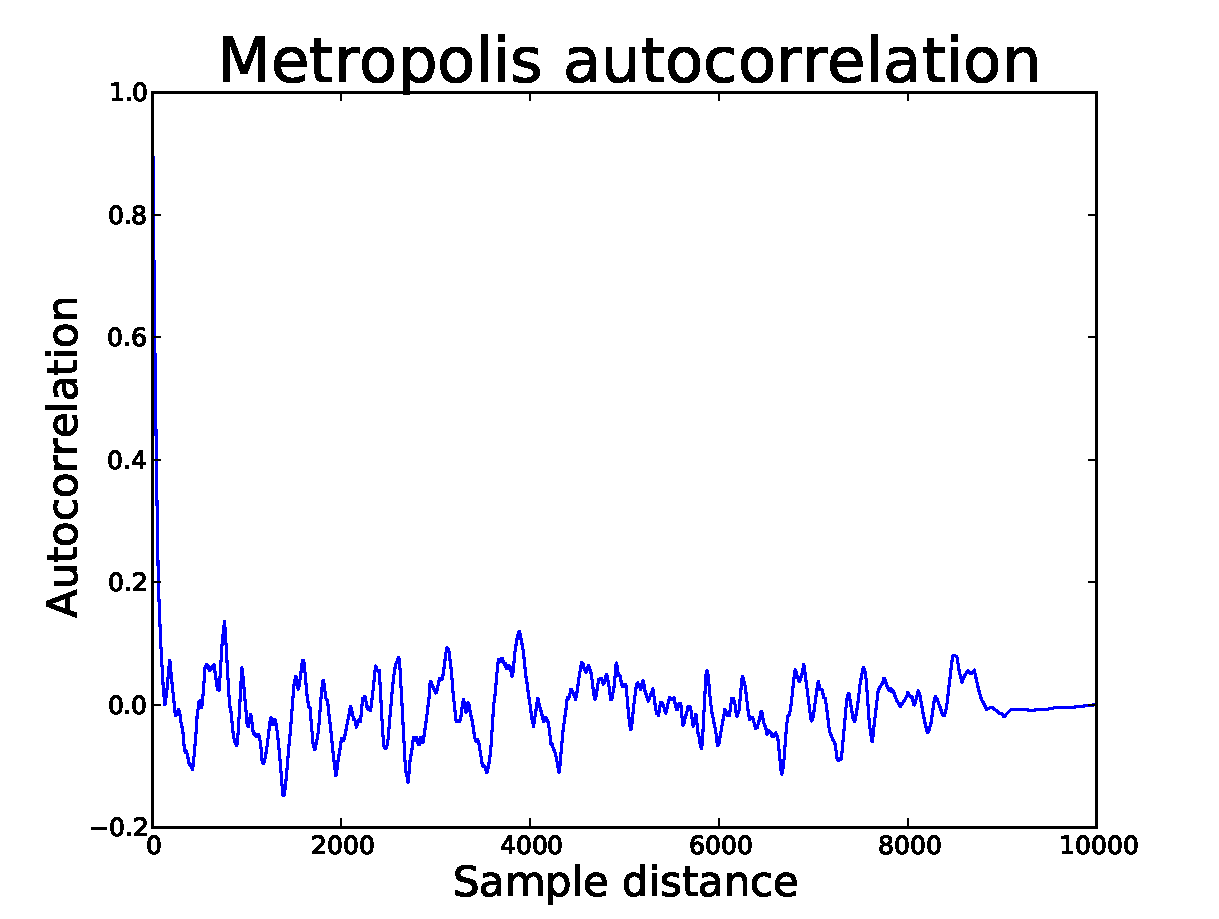
\includegraphics[width=0.8\textwidth]{MetAutoCorr}
    \caption{Sample autocorrelation of the metropolis-hastings algorithm on the Tdf continuous model}
    \label{fig:MetAutoCorr}
\end{figure}

\begin{figure}[H]
    \centering
    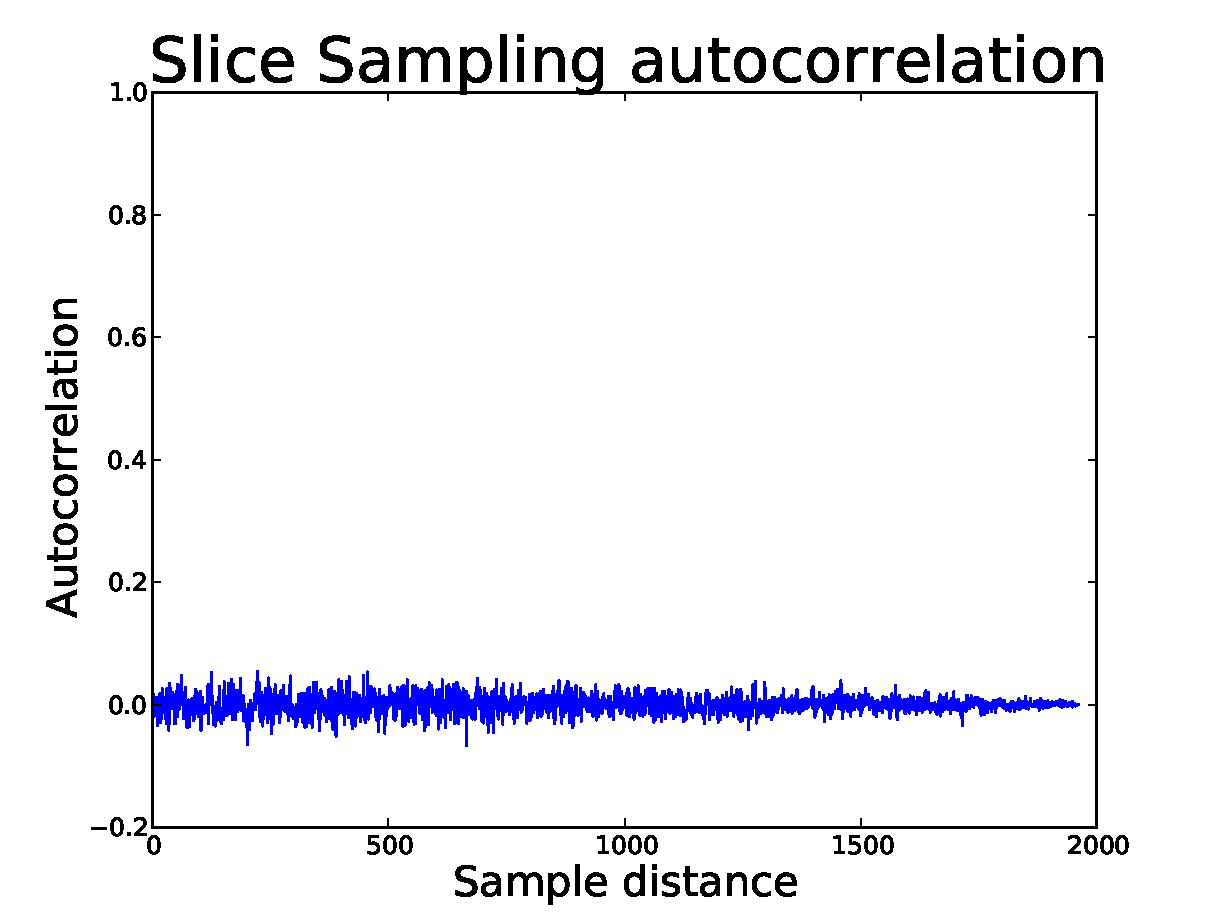
\includegraphics[width=0.8\textwidth]{SliceAutoCorr}
    \caption{Sample autocorrelation of the slice sampling algorithm on the Tdf continuous model}
    \label{fig:SliceAutoCorr}
\end{figure}

\begin{figure}[H]
    \centering
    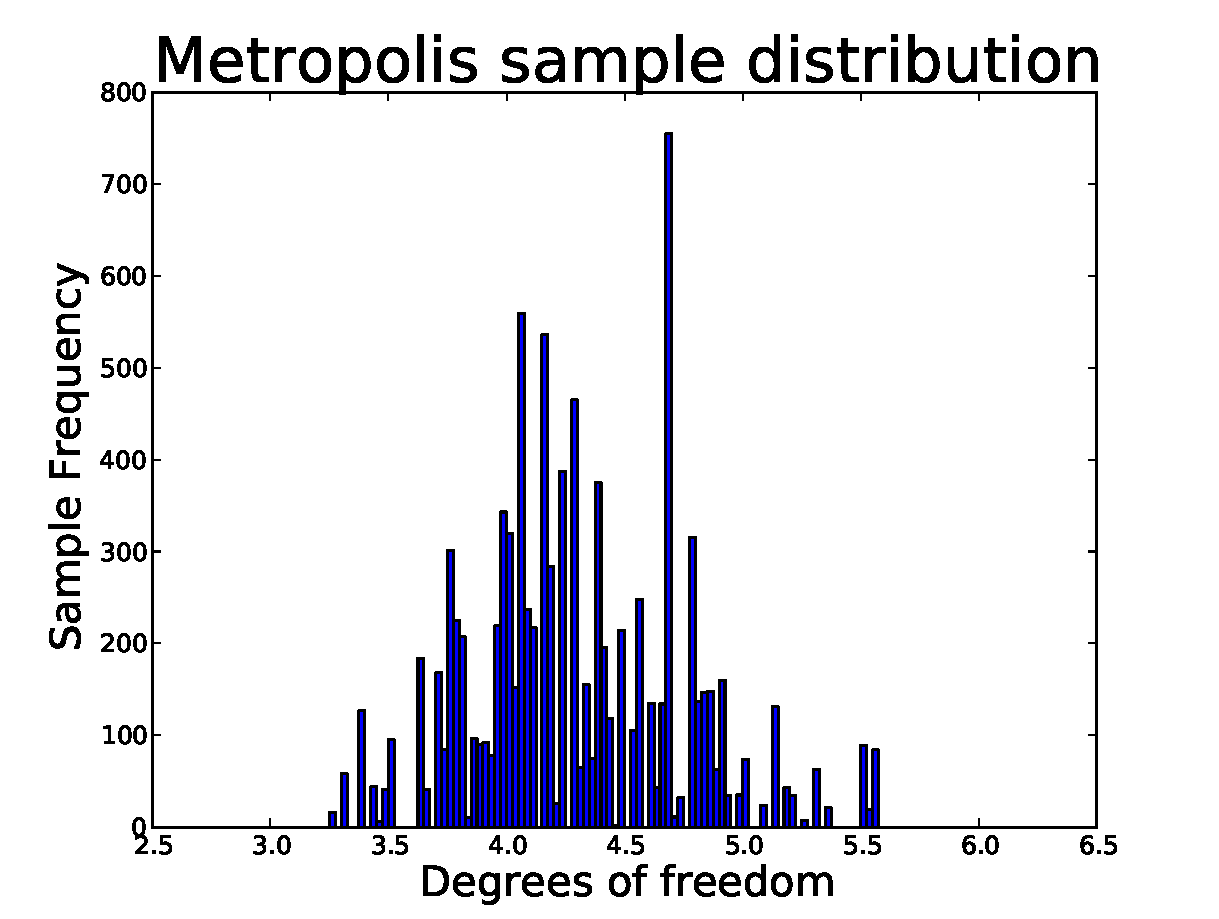
\includegraphics[width=0.8\textwidth]{MetSampDist}
    \caption{Empirical sample distribution of the metropolis-hastings algorithm on the Tdf continuous model}
    \label{fig:MetSampDist}
\end{figure}

\begin{figure}[H]
    \centering
    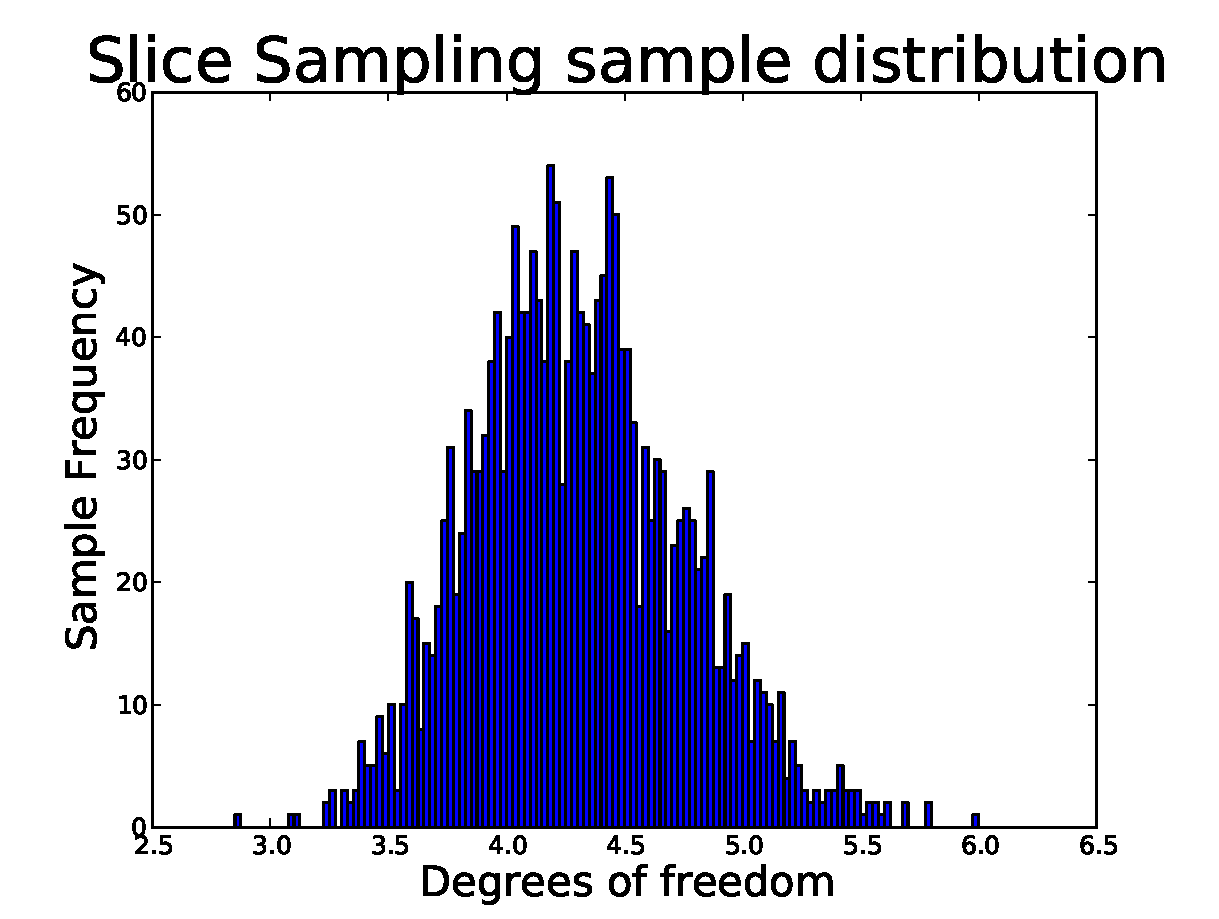
\includegraphics[width=0.8\textwidth]{SliceSampDist}
    \caption{Empirical sample distribution of the slice sampling algorithm on the Tdf continuous model}
    \label{fig:SliceSampDist}
\end{figure}

Based on these preliminary experiments slice sampling seems to confer a significant advantage on the Tdf models.

\subsection{Generic, lightweight, slice sampling inference engine}

Since the custom slice sampling tests on the Tdf models gave promising results we next look at creating a generic slice sampling implementation that can run on arbitrary probabilistic programs. I implemented the procedure in the style of the local metropolis-hastings method presented in the paper “Lightweight Implementations of Probabilistic Programming Languages via Transformational compilation”.

The implementation follows the basic description from Chapter 29.7 in “Information Theory, Inference and Learning Algorithms”. The main points are:
\begin{itemize}

\item
sample a height u in $[0, likelihood]$. Since we are working with log likelihoods that are too small to be exponentiated, we perform the sample directly in logspace by sampling from the exponential corresponding to the log of u. Specifically, if our log likelihood is ll, then $u \sim -1 * (exp(1) + ll)$

\item
sample a random variable x to modify

\item
find values xl and xr smaller and bigger than the current value x of the random variable such that the log likelihood under xl and xr is smaller than the height u (search for these values by doubling the increment value added/subtracted from last guess)

\item
sample proposition for x from uniform(xl, xr), resample until log likelihood under sample is larger than the height u (handling nan log-likelihoods appropriately)

\end{itemize}

The stochastic pythin metropolis implementation presented in Section \ref{sect} runs the Tdf continuous model 2-2.5x slower than the venture implementation. The metropolis implementation also runs about 6x faster than the slice-sampling one per number of samples. As discussed above, the bollteneck is the number of trace likelihood calculations. The metropolis method calculated the log-likelihood exactly once for each sample while slice sampling will execute it a minimum of 3 times (one each for xl, xr and x). In practice, due to the stepping out and the possible resampling of a variable, we average 6 log-likelihood calculations per sample, thus explaining the 6x slow-down.

This shows that, for the tdf model, tweaking the initial width and interval search strategies will result in a further improvement of no more than 2x.

\subsubsection{Slice sampling on Tdf model}
We first run the 3 methods (my custom metropolis and slice sampling implementations and venture) for 10 minutes. The resulting distributions are shown in Figures \ref{fig}, \ref{fig} and \ref{fig}.

\begin{figure}[H]
    \centering
    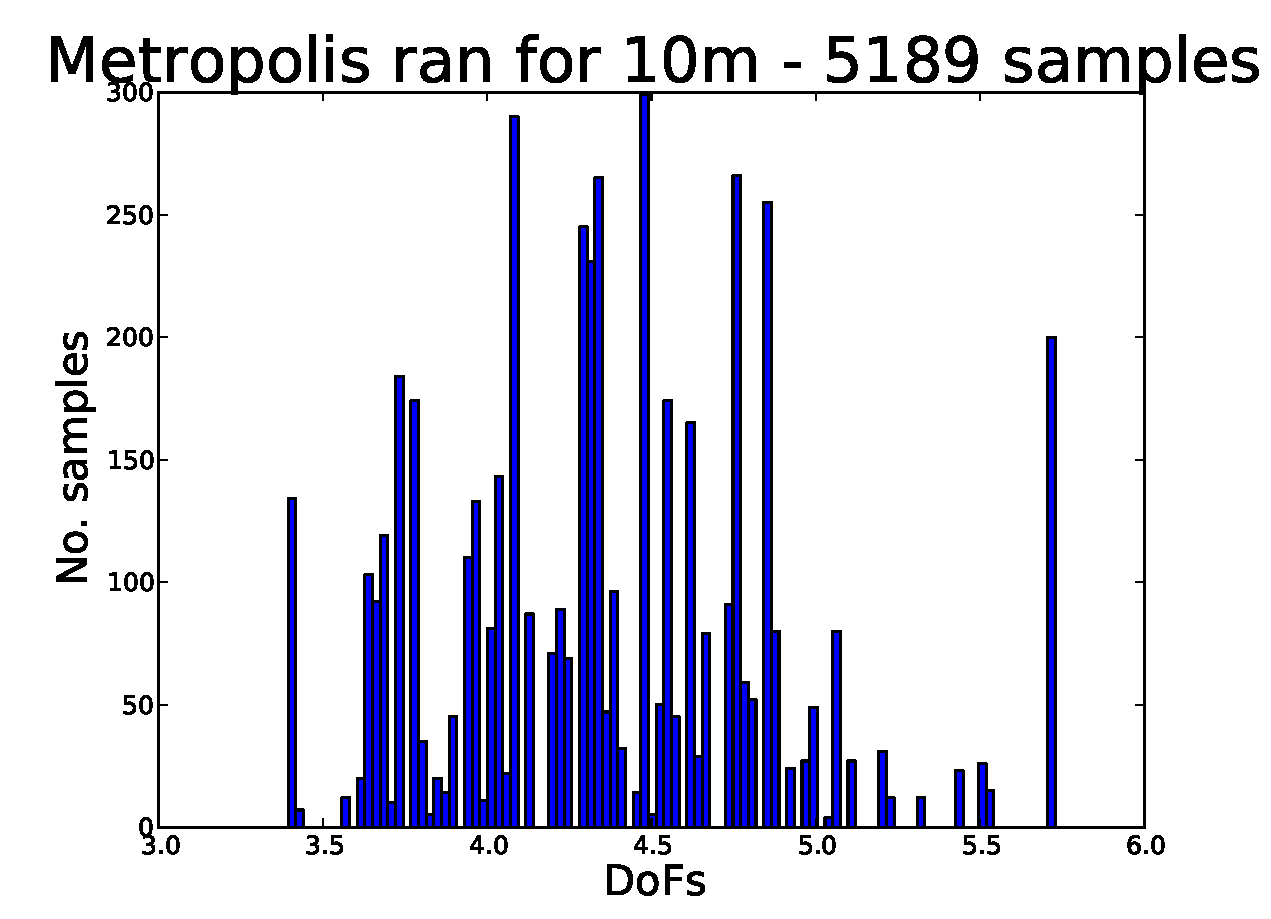
\includegraphics[width=0.8\textwidth]{MetLISampDist}
    \caption{Sample distribution from running custom, lightweight style, Metropolis-Hastings for 10 minutes on Tdf continuous model.}
    \label{fig:MetLISampDist}
\end{figure}

\begin{figure}[H]
    \centering
    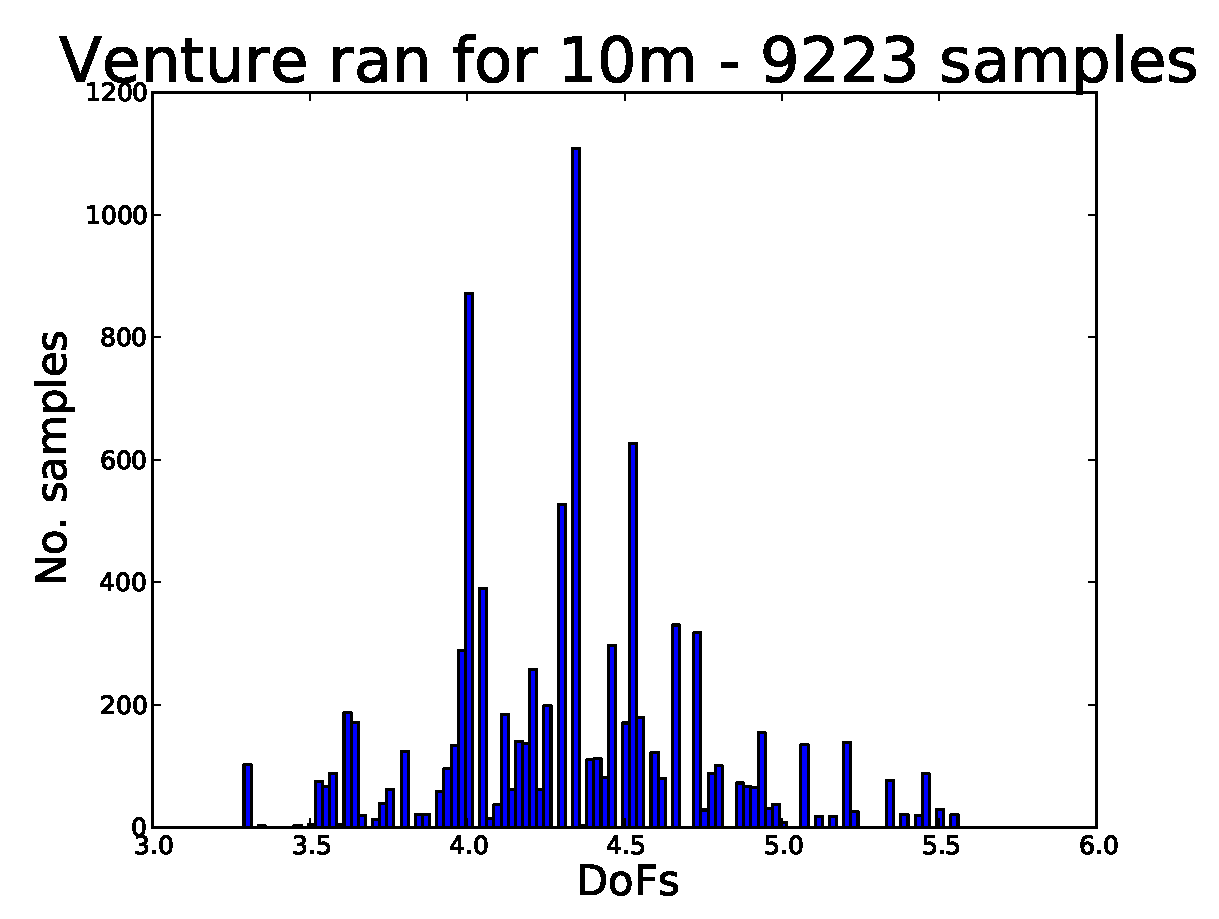
\includegraphics[width=0.8\textwidth]{VentureLISampDist}
    \caption{Sample distribution from running Venture for 10 minutes on Tdf continuous model.}
    \label{fig:VentureLISampDist}
\end{figure}

\begin{figure}[H]
    \centering
    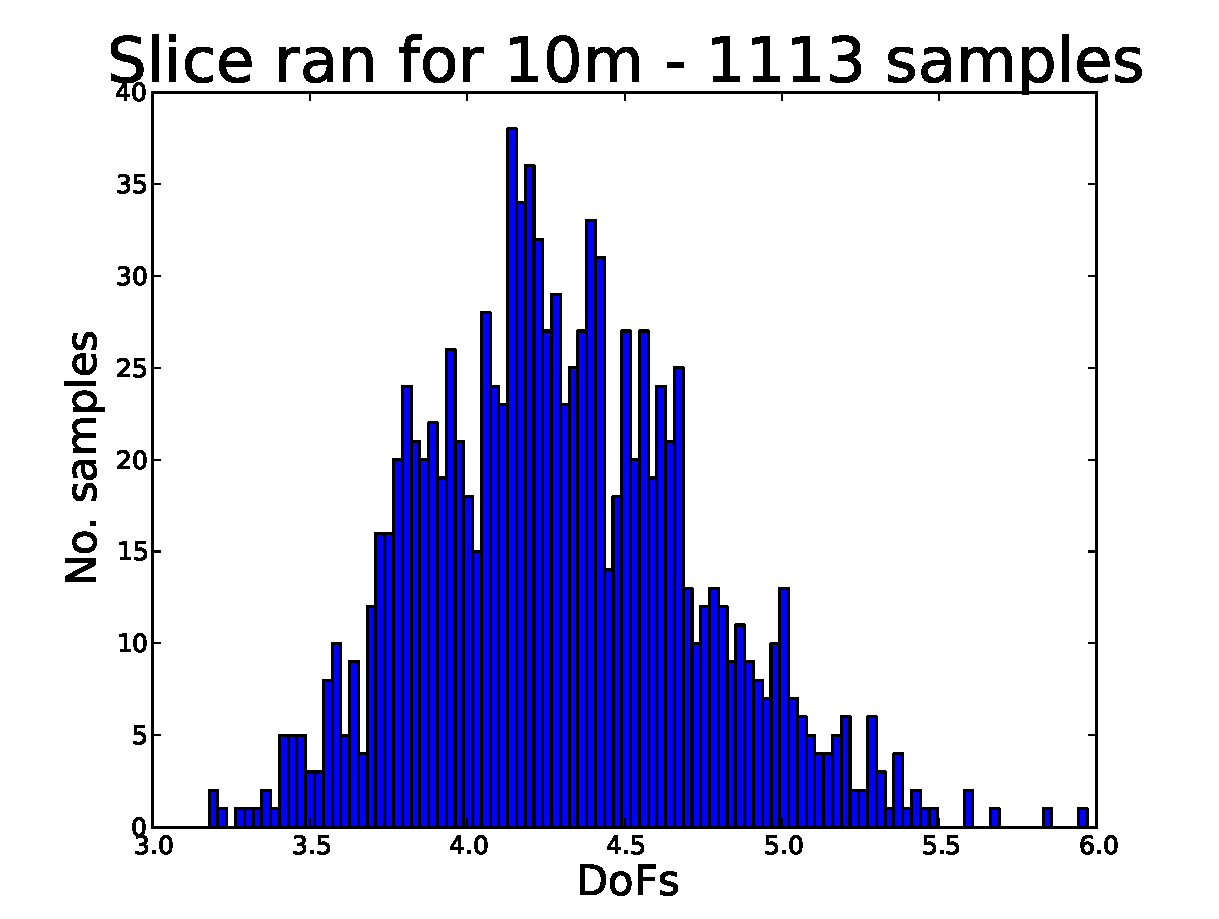
\includegraphics[width=0.8\textwidth]{SliceLISampDist}
    \caption{Sample distribution from running custom, lightweight style, slice sampling for 10 minutes on Tdf continuous model.}
    \label{fig:SliceLISampDist}
\end{figure}

Visually, slice sampling appears to be doing the best job despite generating much fewer samples in 10 minutes than the other methods. In order to get a quantitative evaluation of the methods we can use the Kolmogorov-Smirnov statistic and plot a graph of the decreasing differences between the true cumulative distribution and the cumulative distributions inferred by the 3 methods. This graph (see Figure \ref{fig}) confirms our intuition and show slice sampling significantly outperforming the other variants. 

\begin{figure}[H]
    \centering
    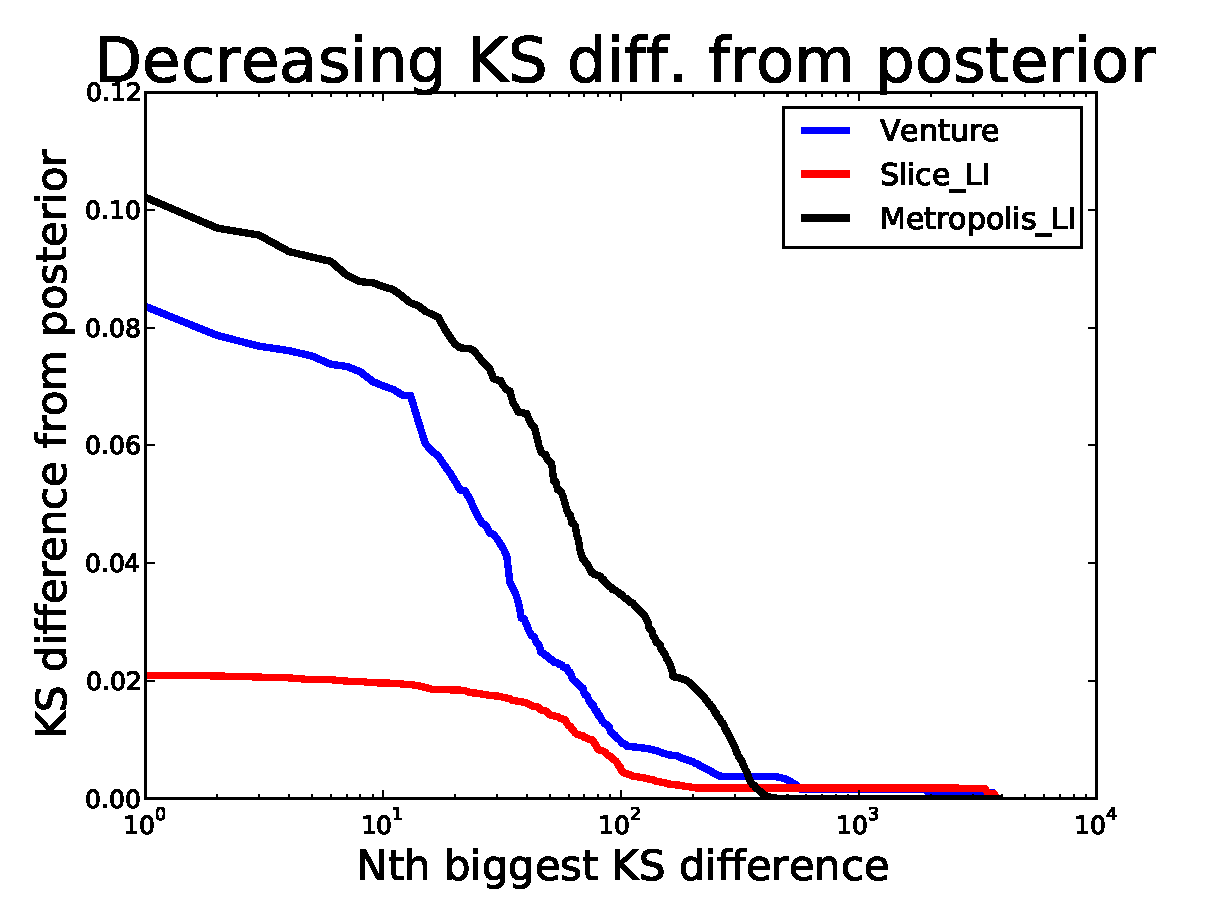
\includegraphics[width=0.8\textwidth]{TdfSliceLIComp}
    \caption{Comparison of decreasing Kolmogorov-Smirnov differences between true and inferred posterior.}
    \label{fig:TdfSliceLIComp}
\end{figure}

\subsubsection{Slice sampling on gaussian mean inference models}
To further test the inference performance of metropolis and slice sampling I defined 3 models based on the problem of estimating the mean of a gaussian. The 3 models are and their posteriors are:

$$
NormalMean1:
m \sim N(0,1)
observe N(m,1) = 5
predict m
$$

\begin{figure}[H]
    \centering
    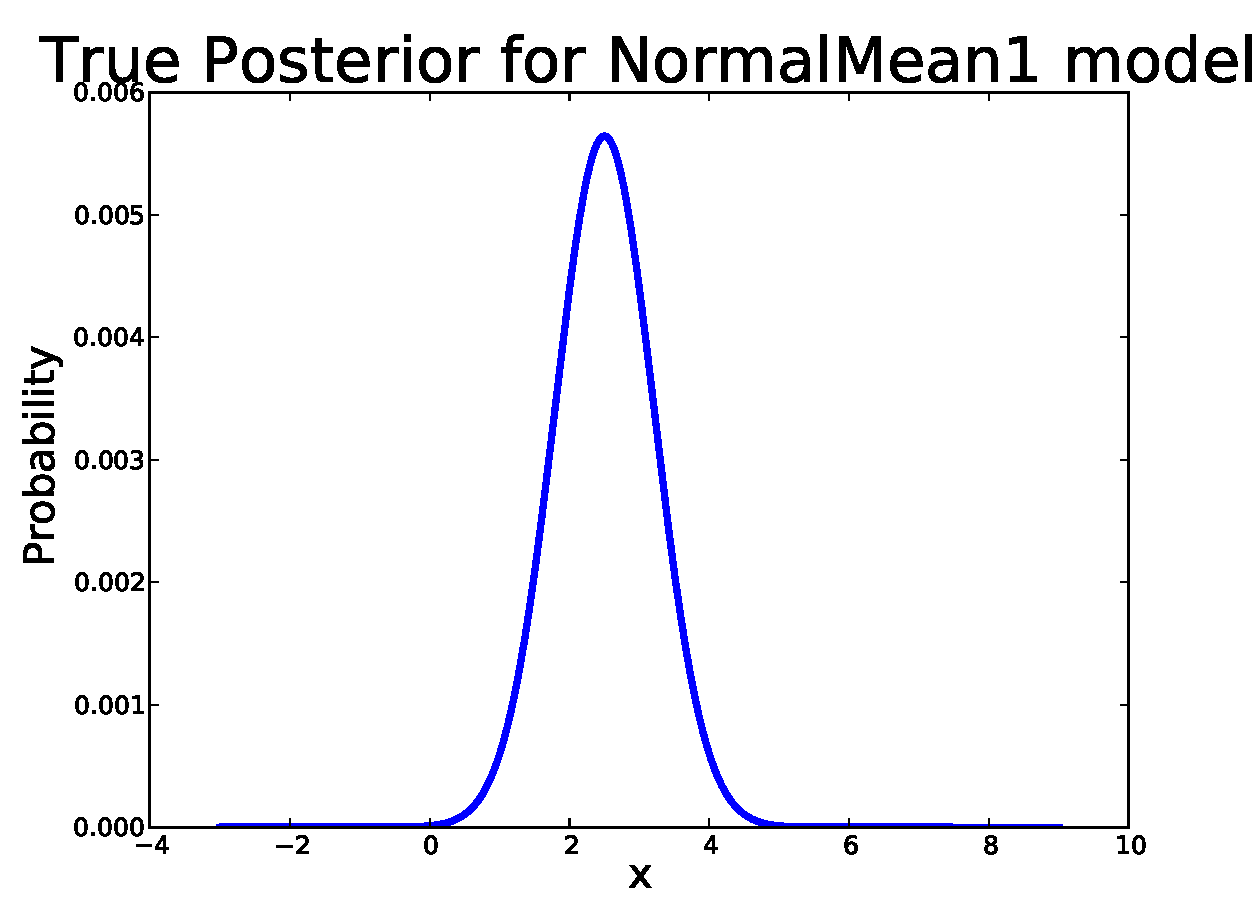
\includegraphics[width=0.8\textwidth]{Normal1Post}
    \caption{Analytically derived posterior for the NormalMean1 model.}
    \label{fig:Normal1Post}
\end{figure}

$$
NormalMean2:
m \sim N(0,1)
v \sim invGamma(3,1)
observe N(m,v) = 5
predict m
$$

\begin{figure}[H]
    \centering
    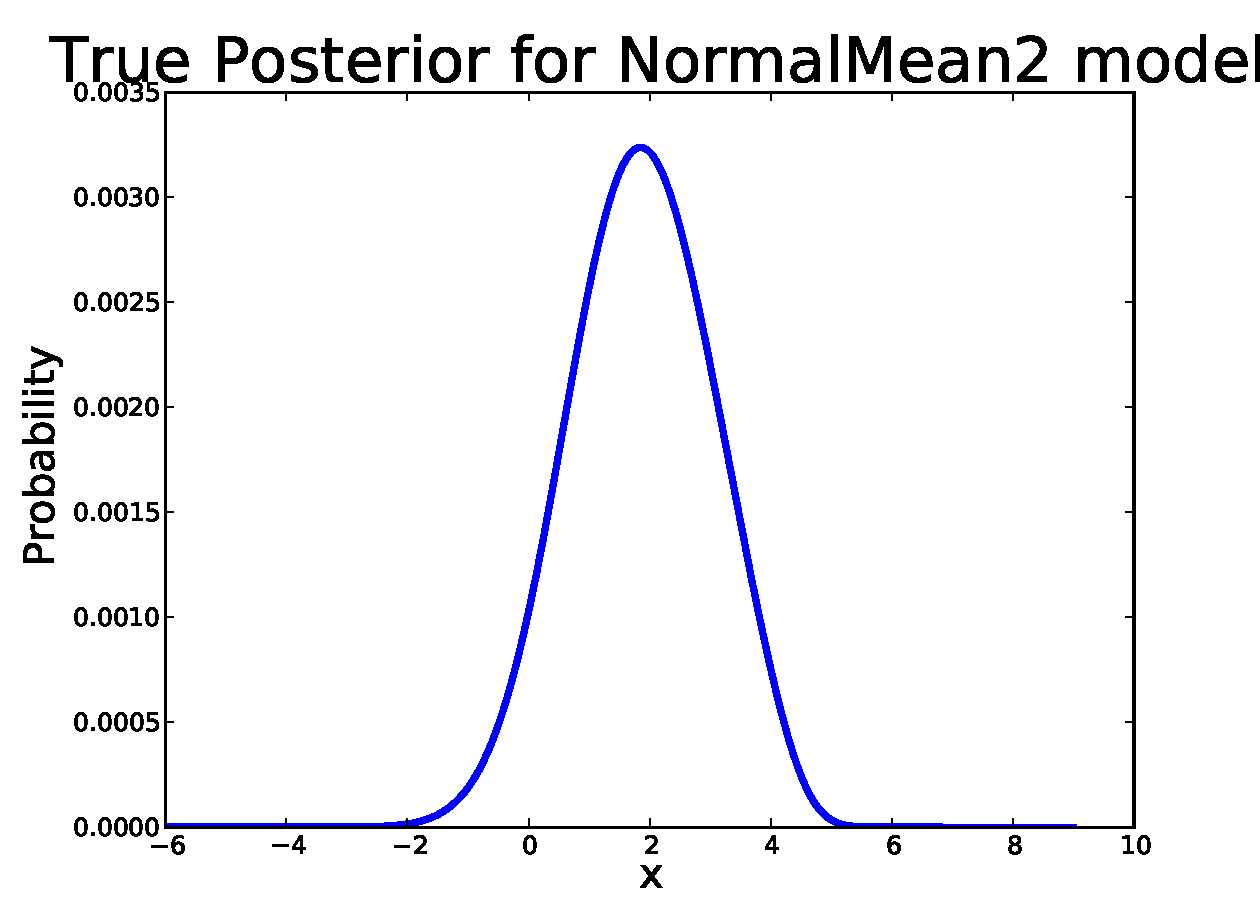
\includegraphics[width=0.8\textwidth]{Normal2Post}
    \caption{Analytically derived posterior for the NormalMean2 model.}
    \label{fig:Normal2Post}
\end{figure}

$$
NormalMean3:
m \sim N(0,1)
if m < 0
    v \sim invGamma(3,1)
else
    v = 1/3
observe N(m,v) = 5
predict m
$$

\begin{figure}[H]
    \centering
    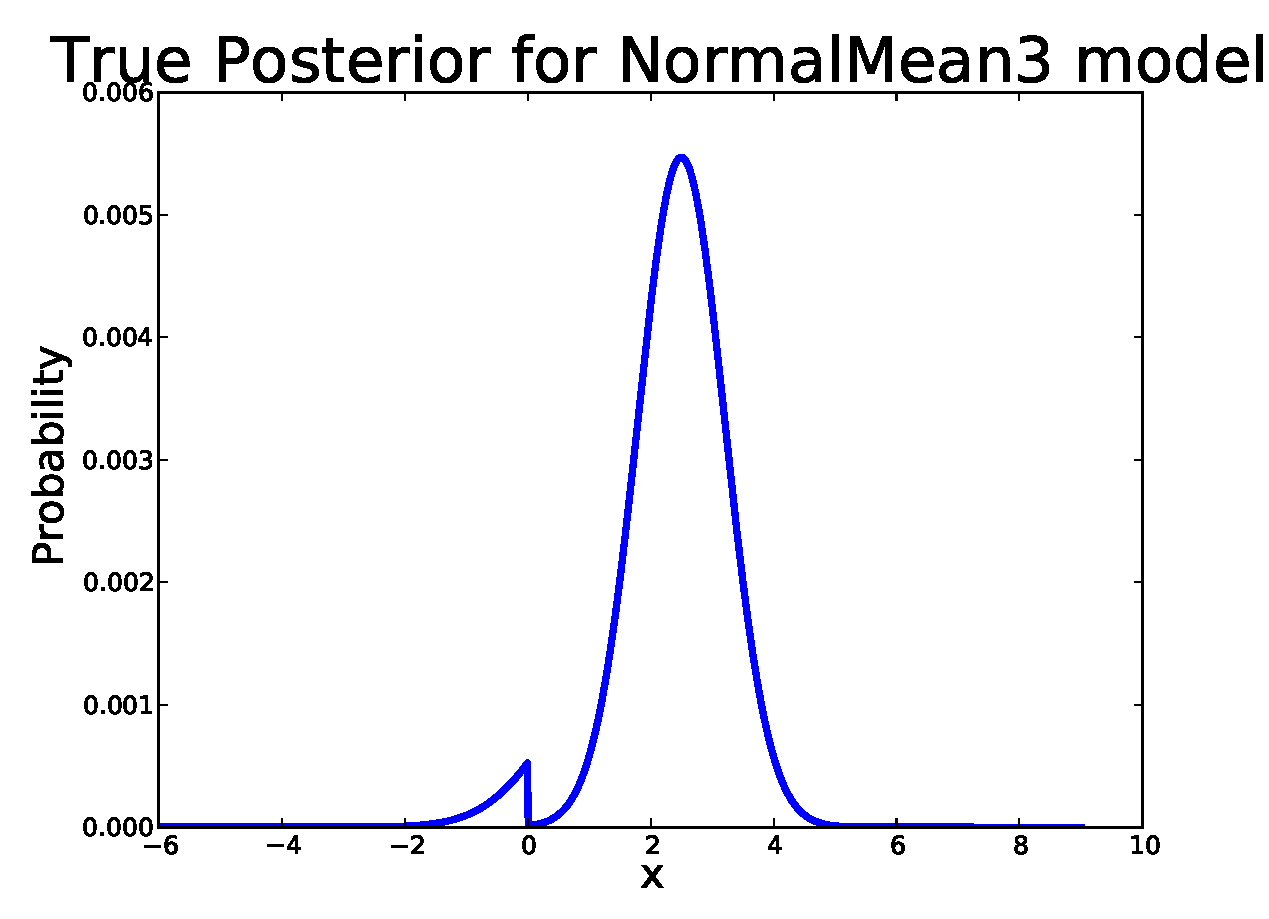
\includegraphics[width=0.8\textwidth]{Normal3Post}
    \caption{Analytically derived posterior for the NormalMean3 model.}
    \label{fig:Normal3Post}
\end{figure}

We now look at the performance of metropolis, slice sampling and a mixture of slice sampling and metropolis (with different mixing weights) over the 3 models. To compare the inference methods we extract samples untill a certain number of trace likelihood calculations are performed. We then compute 100 separate sample runs, starting from 100 different seeds. We consider pure meteropolis-hastings inference, pure slice sampling inference and a combination method that flips a biased coin to decide which inference method to use to extract the next sample.
We plot both all runs generated by the engines on the 3 models as well as the quartiles of these runs.

\begin{figure}[H]
    \centering
    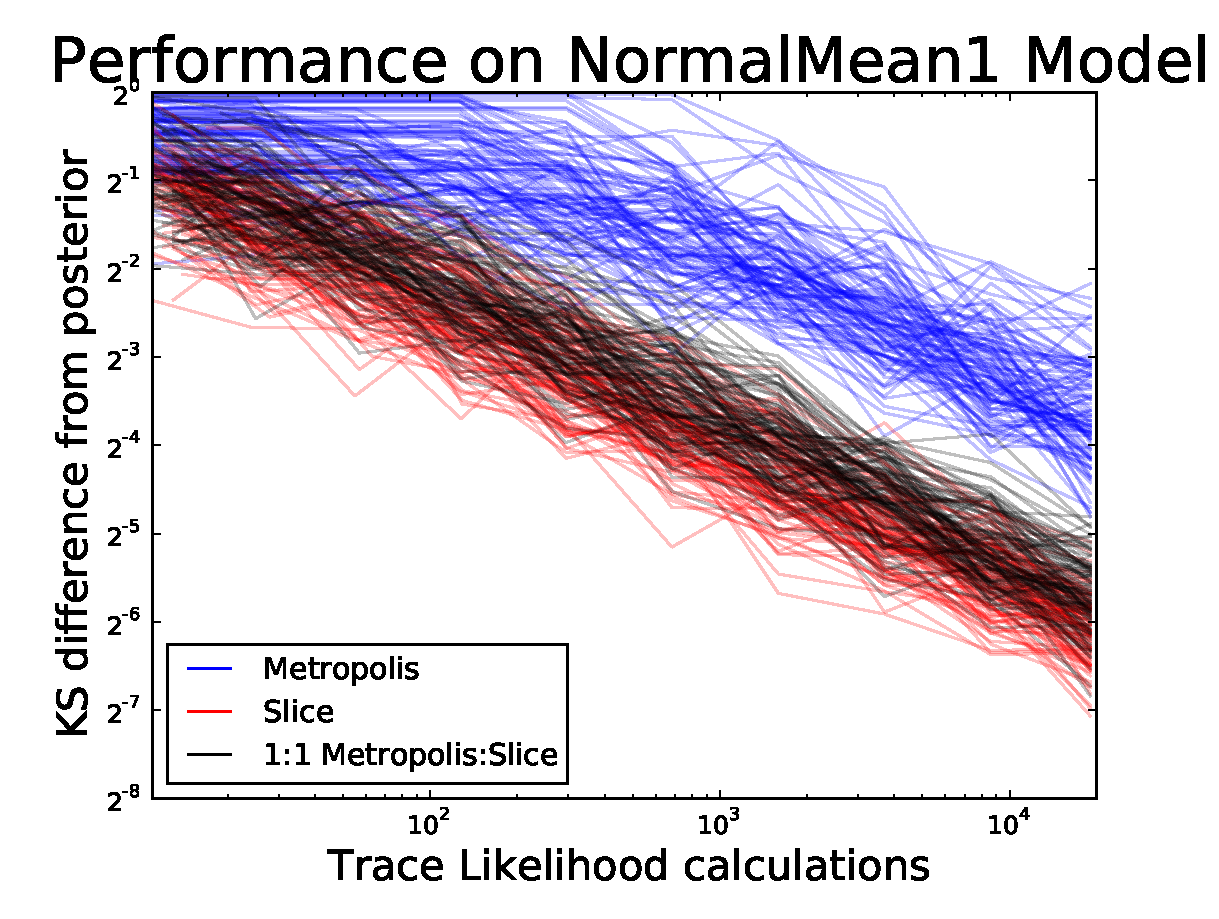
\includegraphics[width=0.8\textwidth]{Normal1Runs}
    \caption{Runs generated by slice, metropolis and an equal mix of metropolis and slice on the 1 dimensional NormalMean1 model.}
    \label{fig:Normal1Runs}
\end{figure}

\begin{figure}[H]
    \centering
    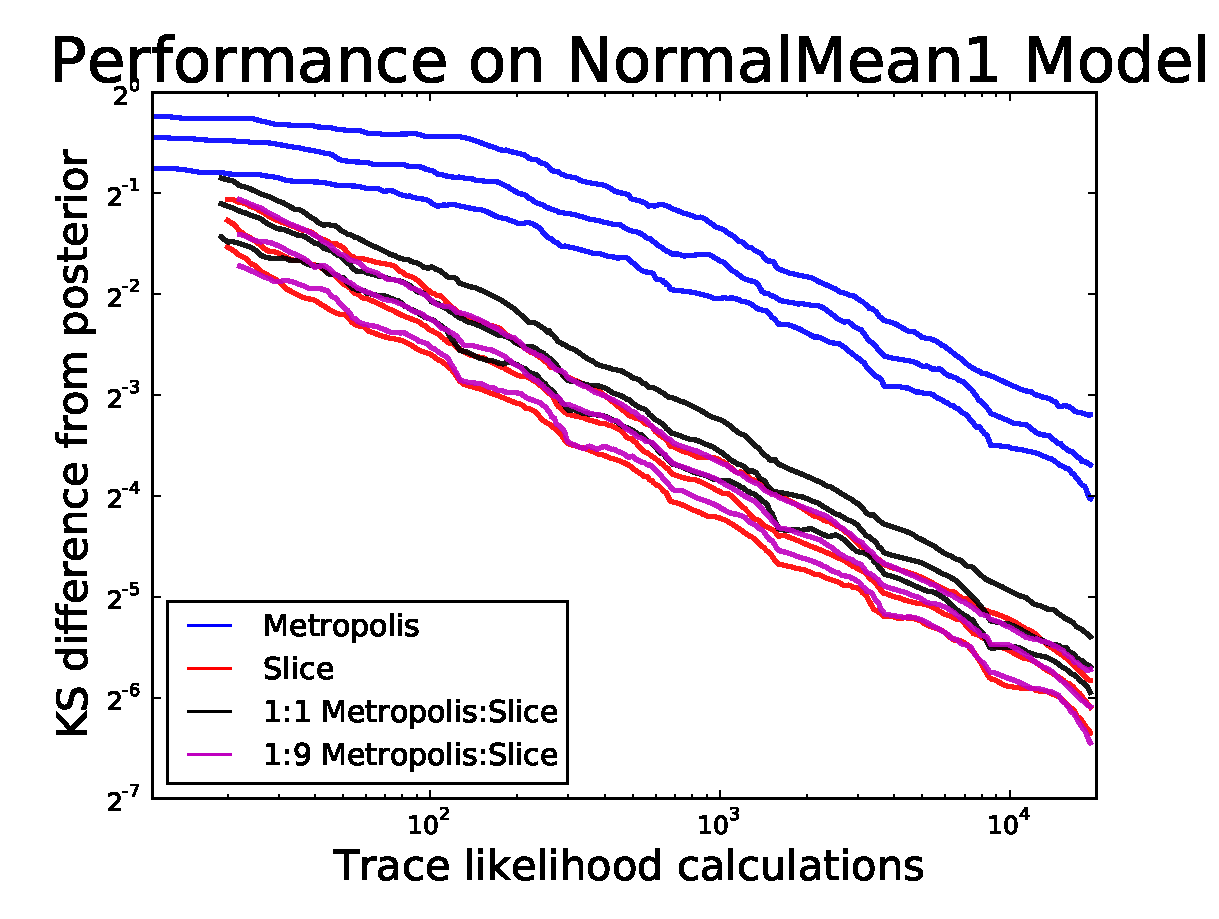
\includegraphics[width=0.8\textwidth]{Normal1Quarts}
    \caption{Quartiles of the runs generated by slice, metropolis and an two different mixes of metropolis and slice on the 1 dimensional NormalMean1 model.}
    \label{fig:Normal1Quarts}
\end{figure}

On the simple, 1d, model all variants of slice sampling clearly outperform metropolis. In the second graph we consider a mixture metropolis and slice both with 10\% metropolis and with 50\% metropolis and find that the change doesn't have a significant impact on performance.
This is likely because, if slice picks good samples, metropolis is likely to simply keep them unchanged (since it will reject the proposal from the prior).

\begin{figure}[H]
    \centering
    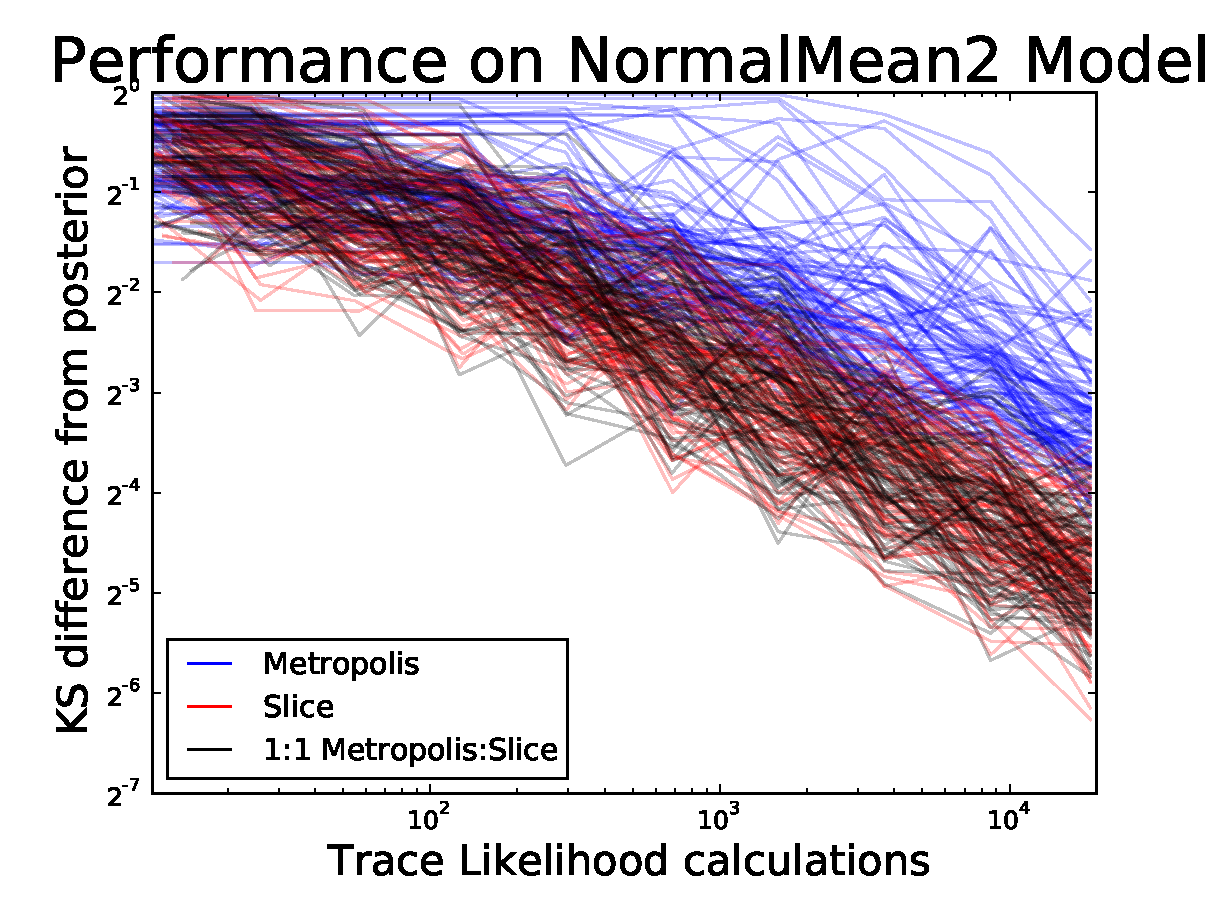
\includegraphics[width=0.8\textwidth]{Normal2Runs}
    \caption{Runs generated by slice, metropolis and an equal mix of metropolis and slice on the 2 dimensional NormalMean2 model.}
    \label{fig:Normal2Runs}
\end{figure}

\begin{figure}[H]
    \centering
    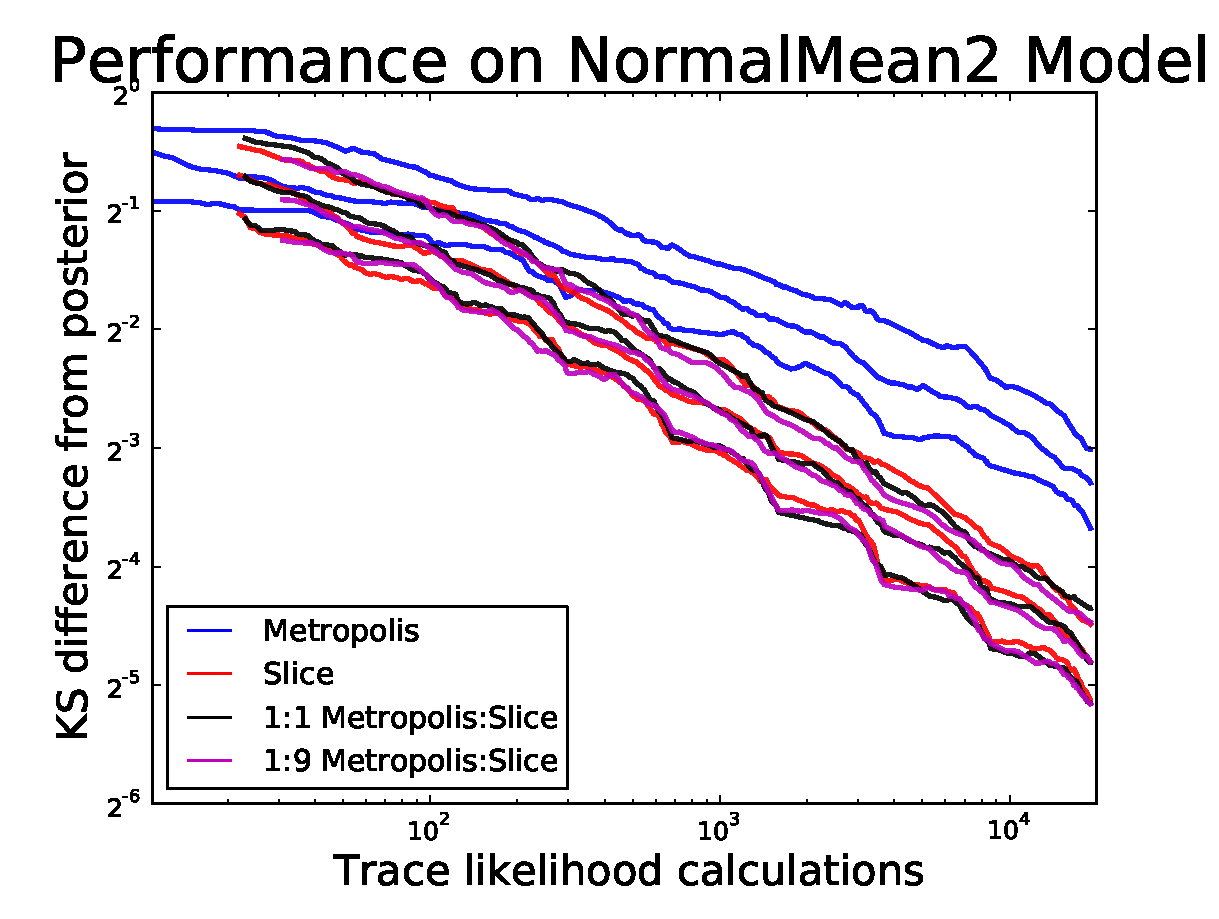
\includegraphics[width=0.8\textwidth]{Normal2Quarts}
    \caption{Quartiles of the runs generated by slice, metropolis and an two different mixes of metropolis and slice on the 2 dimensional NormalMean2 model.}
    \label{fig:Normal2Quarts}
\end{figure}

On the 2d model, slice still clearly outperforms metropolis, though the gap is not as pronounced as for the 1d model. Further the observation from the 1d model still holds and the 3 different slice variants all get quite similar performance. Actually, on this model, the fact that the slice mixtures get more samples per LL calculation translates into a slightly better performance for them than for the pure slice sampling method.

\begin{figure}[H]
    \centering
    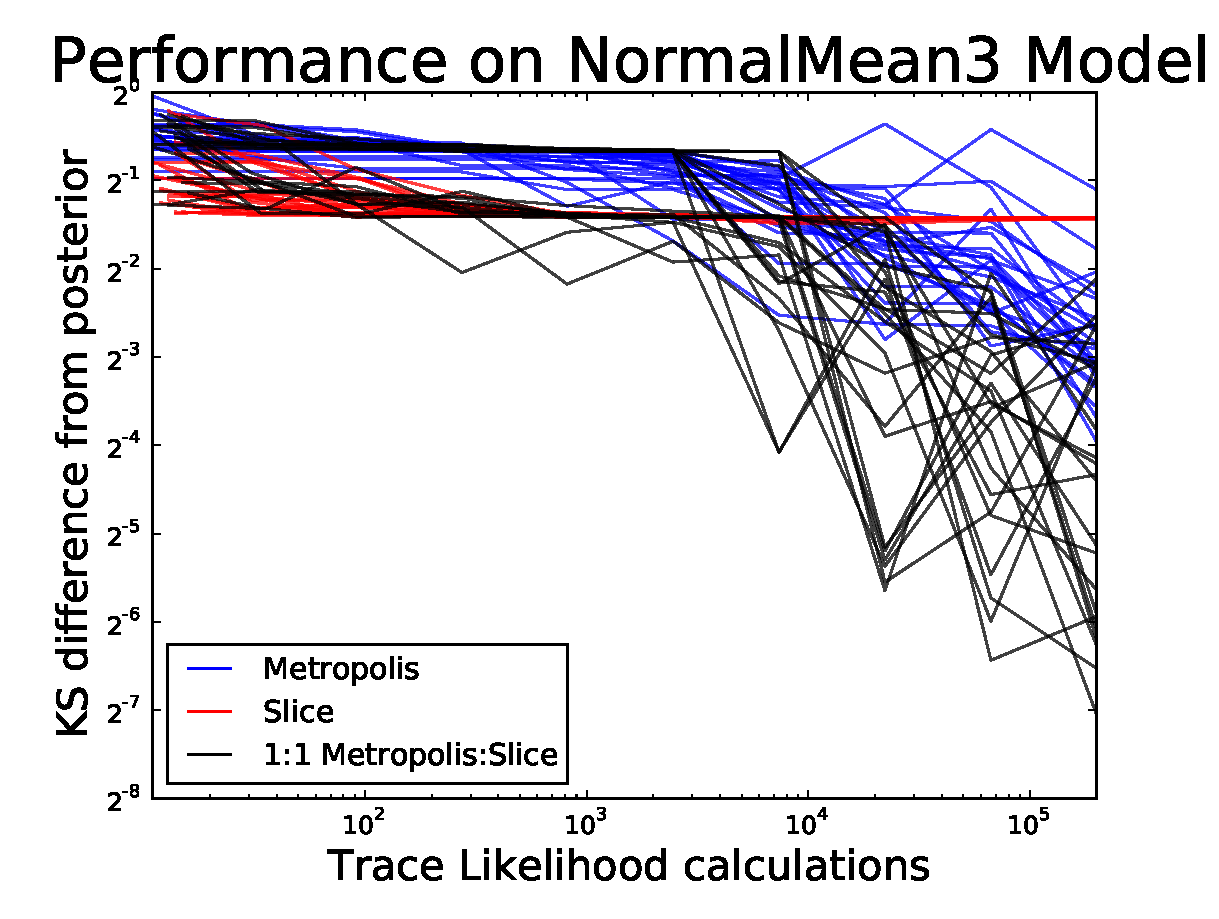
\includegraphics[width=0.8\textwidth]{Normal4Runs}
    \caption{Runs generated by slice, metropolis and an equal mix of metropolis and slice on the trans-dimensional NormalMean3 model.}
    \label{fig:Normal4Runs}
\end{figure}

\begin{figure}[H]
    \centering
    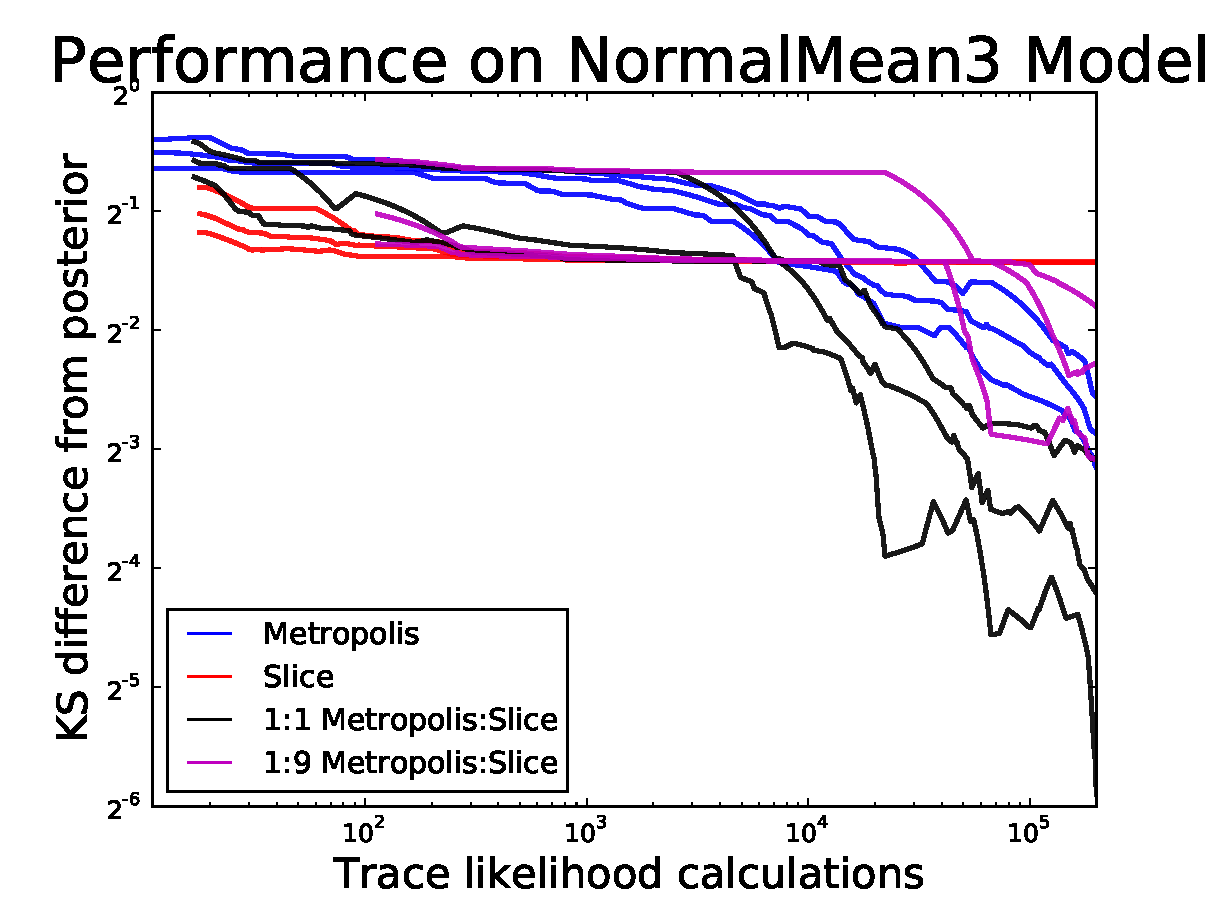
\includegraphics[width=0.8\textwidth]{Normal4Quarts}
    \caption{Quartiles of the runs generated by slice, metropolis and an two different mixes of metropolis and slice on the trans-dimensional NormalMean3 model.}
    \label{fig:Normal4Quarts}
\end{figure}

On this third model there are several things worth noting. First of all, pure slice sampling does very badly. This is because the simple slice sampling algorithm used in this example cannot handle trans-dimensional probabilistic models, such as NormalMean3. We will look closer at this problem in Sections \ref{sec} and \ref{sec}. 
Further, on this model we see the first significant performance difference between the different mixtures of slice and metropolis. Since slice sampling cannot handle trans-dimensional jumps, one of the main purposes of the metropolis steps in the mixture model is to switch between program traces with different dimensionality. In the case of the 1:9 Metropolis:Slice mixture, we see that this dimensionality switch happens quite rarely, and so the markov chain is stuck on bad samples for long runs. The 1:1 mixture of slice sampling and metropolis, however manages to switch dimensionality sufficiently often and outperforms pure metropolis.


\subsubsection{Branching Model}

In order to further test the slice sampling inference engine we look at the Branching model from the paper ``A New Approach to Probabilistic Programming Inference''. This is also a trans-dimensional model, but this time operating on discrete data. The model specification I use is:

$$
Branching3:
pois1 \sim Poisson(4)
if r > 4
    x = 6
else
    pois2 \sim Poisson(4)
    x = fib(3 * pois1) + pois2
observe Poisson(x) = 6
predict pois1
$$

Where $fib$ is the fibonacci function. \todo{mention the discrepancy with the paper?}

In order to test the convergence rate of the inference engines we must first analytically derive the true posterior for this model. This is given, up to values of 20 in Figure \ref{fig}

\begin{figure}[H]
    \centering
    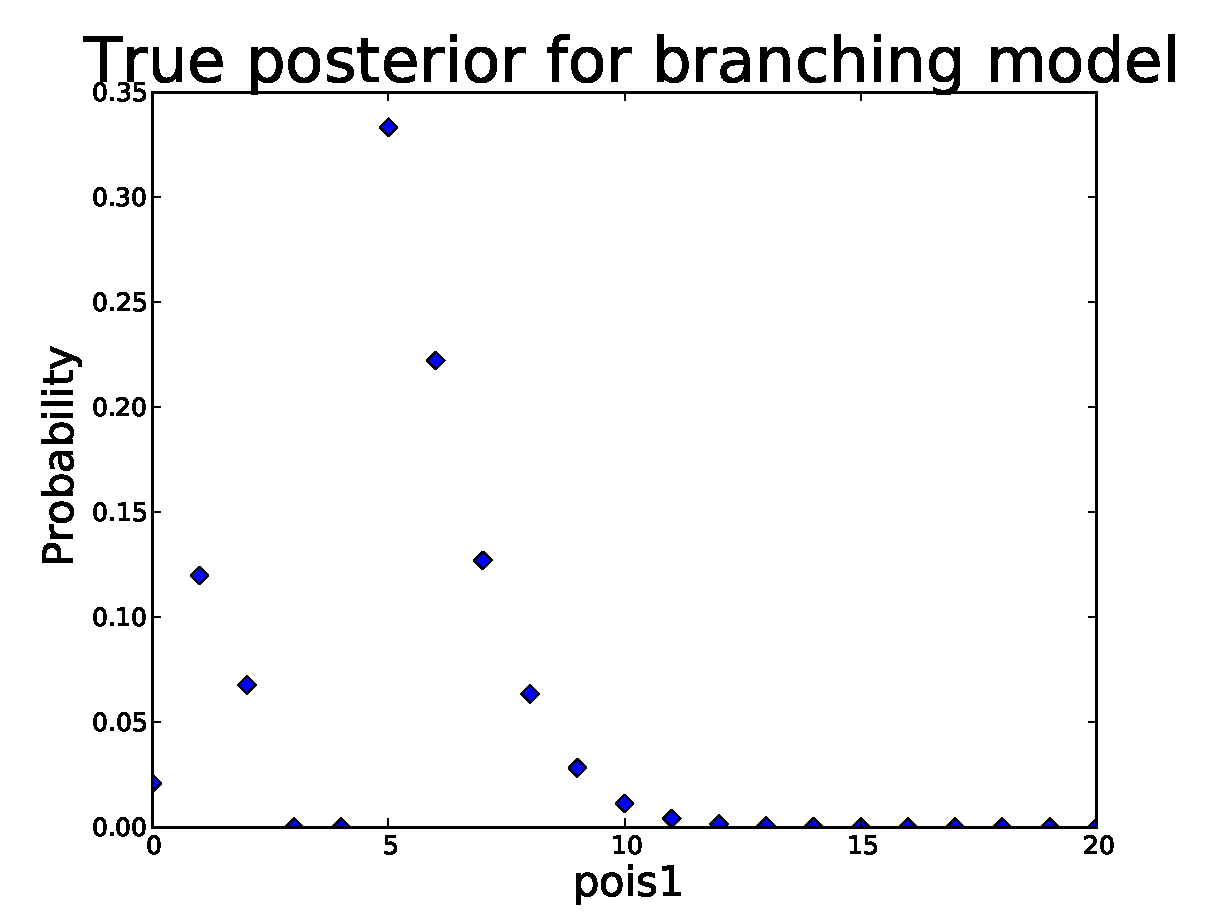
\includegraphics[width=0.8\textwidth]{BranchPost}
    \caption{True posterior for the Branching Model}
    \label{fig:BranchPost}
\end{figure}

In order to evaluate the engines, we generate 100 traces with both inference methods and plot the evolution of the KL divergence relative to the analytical posterior as the number of trace likelihood increases. Using trace likelihood calculations instead of number of samples means that the different methods are comparable since the trace likelihood calculation is the computational bottleneck.

\begin{figure}[H]
    \centering
    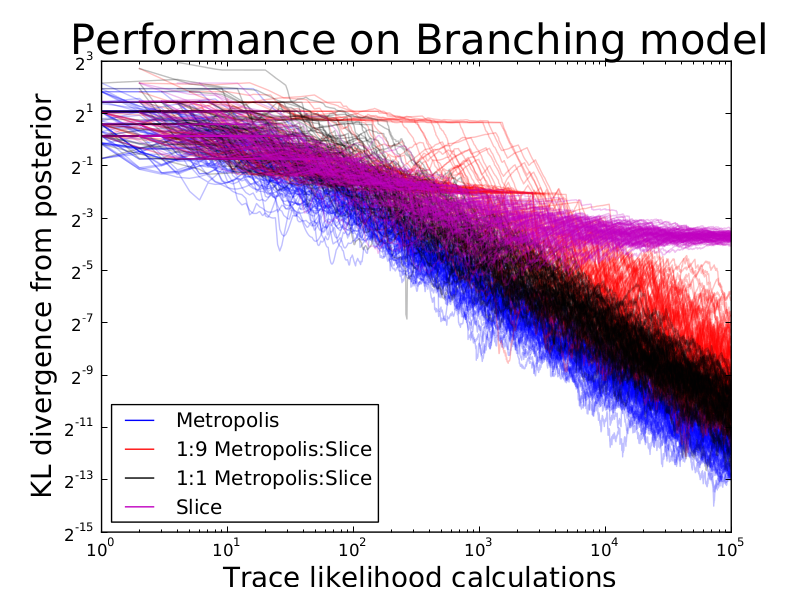
\includegraphics[width=0.8\textwidth]{BranchRuns}
    \caption{Runs generated by slice, metropolis and two mixtures of metropolis and slice on the Branching model.}
    \label{fig:BranchRuns}
\end{figure}

\begin{figure}[H]
    \centering
    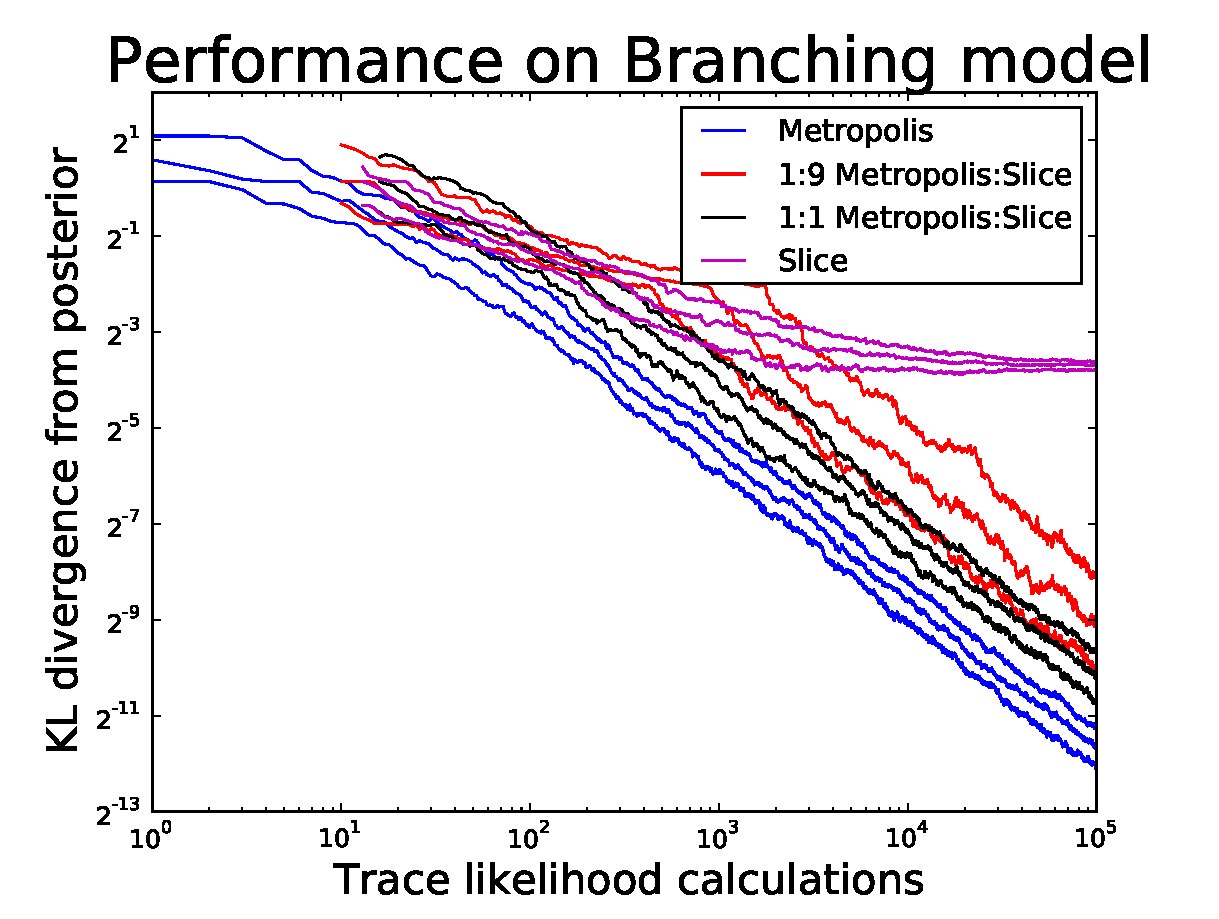
\includegraphics[width=0.8\textwidth]{BranchQuarts}
    \caption{Quartiles of the runs generated by slice, metropolis and two mixtures of metropolis and slice on the Branching model.}
    \label{fig:BranchQuarts}
\end{figure}

As for the previous trans-dimensional model (NormalMode3), we see that the slice inference does not converge to the correct distribution since it cannot handle trans-dimensional jumps. The Metropolis:Slice mixtures do converge correctly but, on this model, are less efficient than the local Metropolis-Hastings.

One thing worth noting on this model is that slice sampling proposes some values of pois1 that are extremely unlikely (such as 60). The reason it proposes these values is that it picks a slice height based on the trace log-likelihood which in this model can be extremely low due to the distribution of the conditioned upon x variable. In the Branching model, likely values of the 2 random variables (based on their priors) can result in very unlikely program traces and these traces can then result in accepting very unlikely values of our 2 random variables, since the acceptance criterion is simply that the proposed trace have likelihood higher than a number drawn uniformly from [0, oldTraceLL]

However, we would expect this behaviour to only occur at the begining of a run, so the 1000 trace likelihood calculations burn-in period we are using should mitigate any influence this factor may have.

It's also unclear why slice does worse on this model than on the NormalMean3 one. One difference between the 2 models is that the slice sampling in the branching model ends up proposing (and thus refusing) more trans-dimensional samples than the NormalMean3 model. When calculating 100,000 model simulations, branching gets about 12,500 rejected trans-dimensional jumps while NormalMean3 only gets about 4,500. However the overall efficiency of the slice/metropolis mix doesn't seem to be affected, as both models average about 1 sample for 5 LL calculations. \todo{talk about the continuous vs. discrete aspect and the domain in which we expect slice to be good}

It is informative to look at a per sample comparison of the two methods, in addition to the previous per trace likelihood compatrison (even though slice does ``more work'' to generate a sample than metropolis).

\begin{figure}[H]
    \centering
    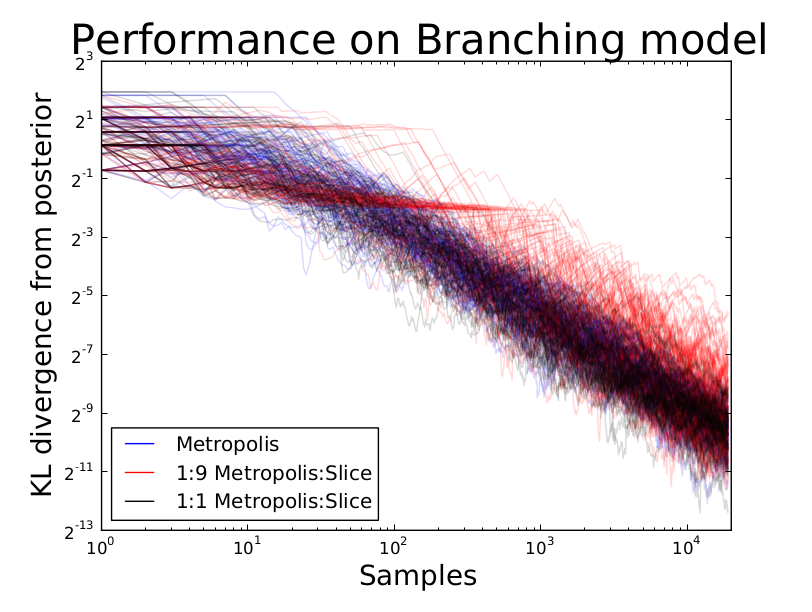
\includegraphics[width=0.8\textwidth]{BranchRunsSamps}
    \caption{Runs generated by metropolis and two mixtures of metropolis and slice on the Branching model.}
    \label{fig:BranchRunsSamps}
\end{figure}

\begin{figure}[H]
    \centering
    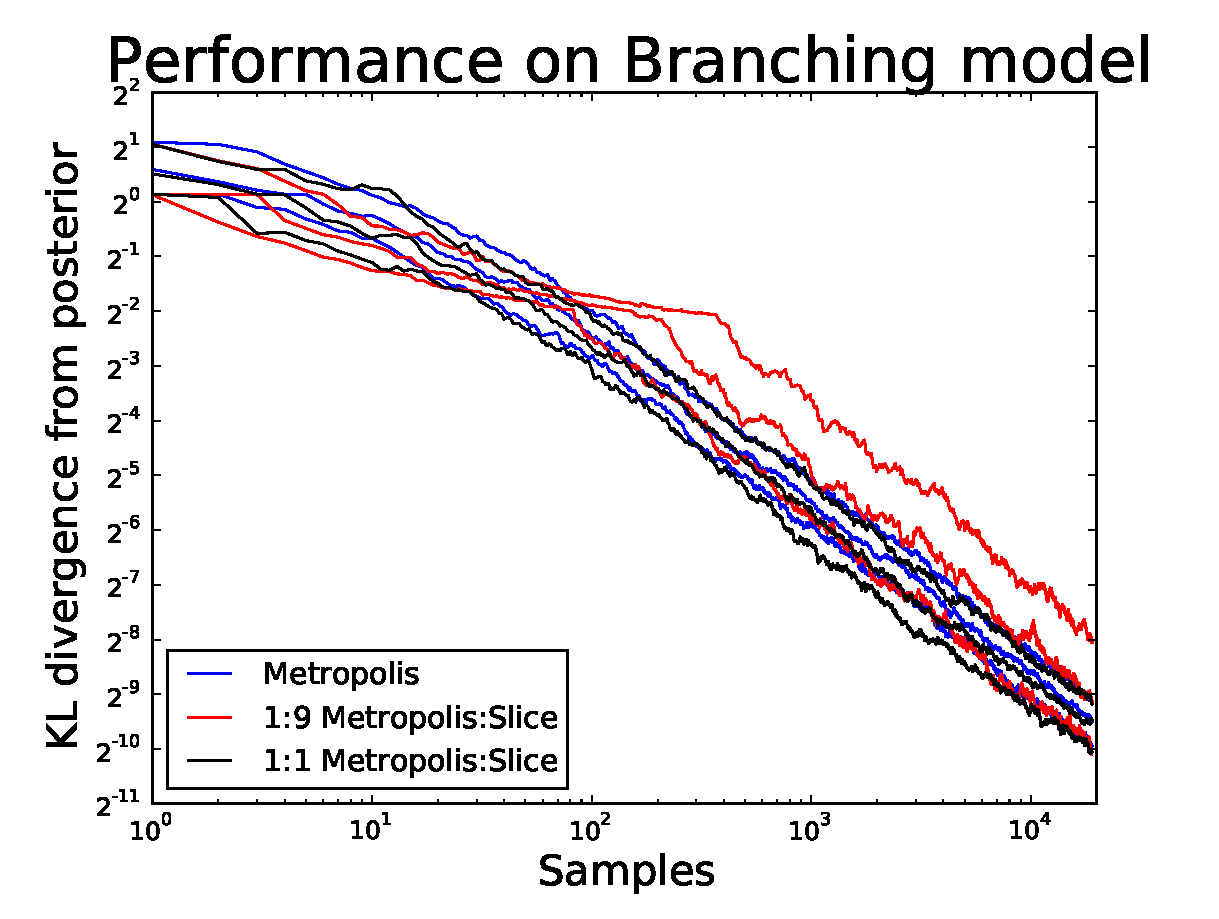
\includegraphics[width=0.8\textwidth]{BranchQuartsSamps}
    \caption{Quartiles of the runs generated by metropolis and two mixtures of metropolis and slice on the Branching model.}
    \label{fig:BranchQuartsSamps}
\end{figure}

Here we can see that the samples generated by 1:1 Metropolis:Slice are actually slightly better than the pure metropolis ones. However the difference is not large enough to make up for the extra trace likelihood calculations that slice sampling must perform. We can also notice that the slice sampling mixtures experience a larger variance in performance than the pure metropolis method. This may be due to the fact that we are relying on only the metropolis generated samples to randomly switch between the 2 modes.

\subsubsection{Trans-dimensional slice sampling}

An interesting research question is whether (and how) it might be possible to modify the slice sampling algorithms so that it can correctly perform inference on probabilistic programs with varying numbers of dimensions.

As a pre-requisite to approaching this question, it is usefull to investigate a little closer what is going wrong when trying to perform inference on these models. Turning back to the Branching model investigated in Section \ref{sec}, we see that the model has 2 random variables whose values determine the distribution of a third variable which we condition on. Additionally, the model is trans-dimensional since on different traces either one or both of these 2 variables will be sampled.

Re-writing the model so that both variables are always sampled, even if one of them is unused, leaves the posterior invariant. Therefore one method to correctly perform inference in a treans-dimensional model is to always sample all the variables that might ever be used in any trace. Of course this will be extremely inneficient in large models and is not a viable solution. We can however use this trick to see what the space of possible trace likelihoods looks like (see Figure \ref{fig}).

\begin{figure}[H]
    \centering
    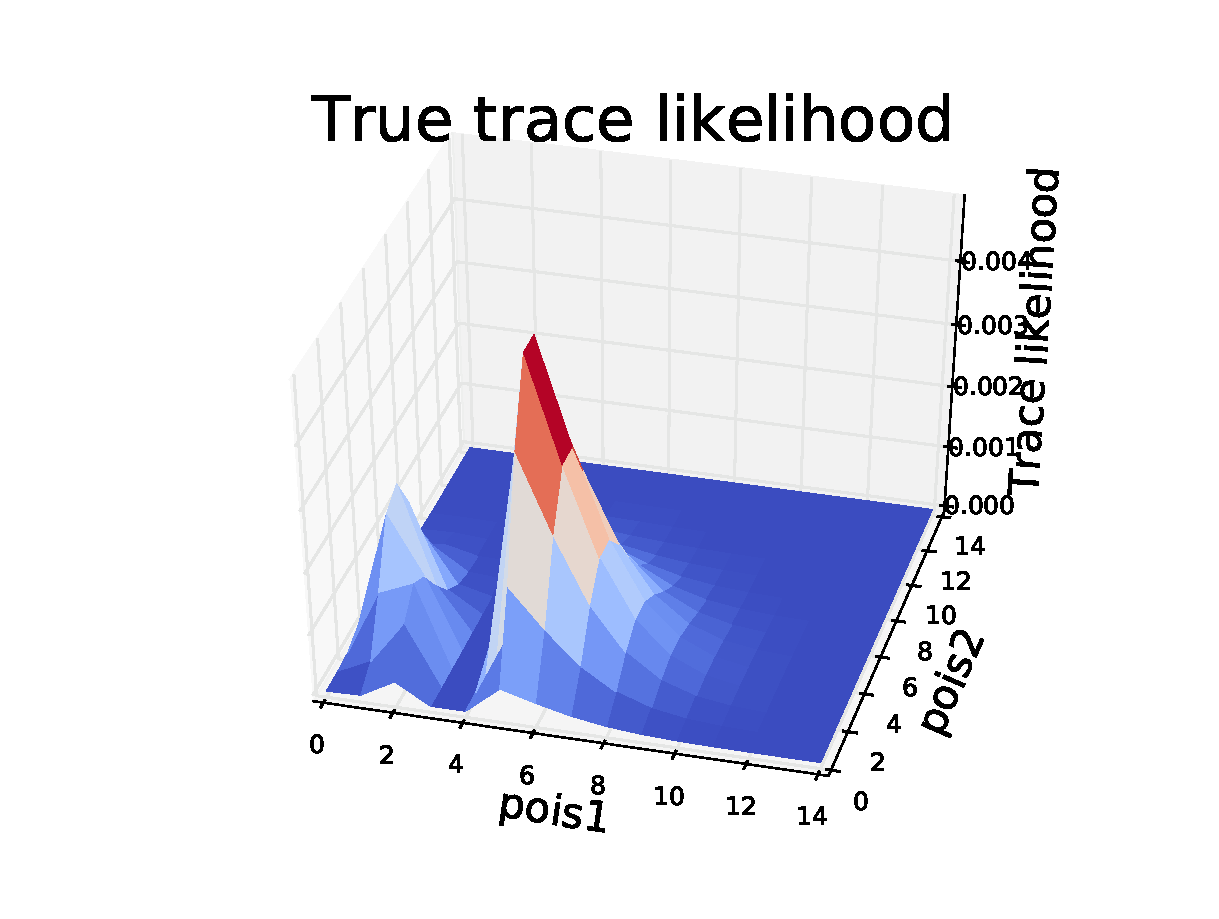
\includegraphics[width=0.8\textwidth]{BranchTraceLik}
    \caption{Space of trace likelihoods if both variables are always sampled.}
    \label{fig:BranchTraceLik}
\end{figure}

Integrating out the pois2 variable from the above trace likelihood space results in the correct posterior distribution (shown in Figure \ref{Fig}).

The naive slice sampling, however, will not sample the second poisson when it is not necessary, but will still think that the trace likelihoods between runs with different numbers of sampled variables are comparable. In doing so, the slice sampler will be pretending to be pretending to be sampling from a 2D trace likelihood even when it really is 1D. The space of likelihoods implied by the naive slice sampling implementation is shown in Figure \ref{fig}

\begin{figure}[H]
    \centering
    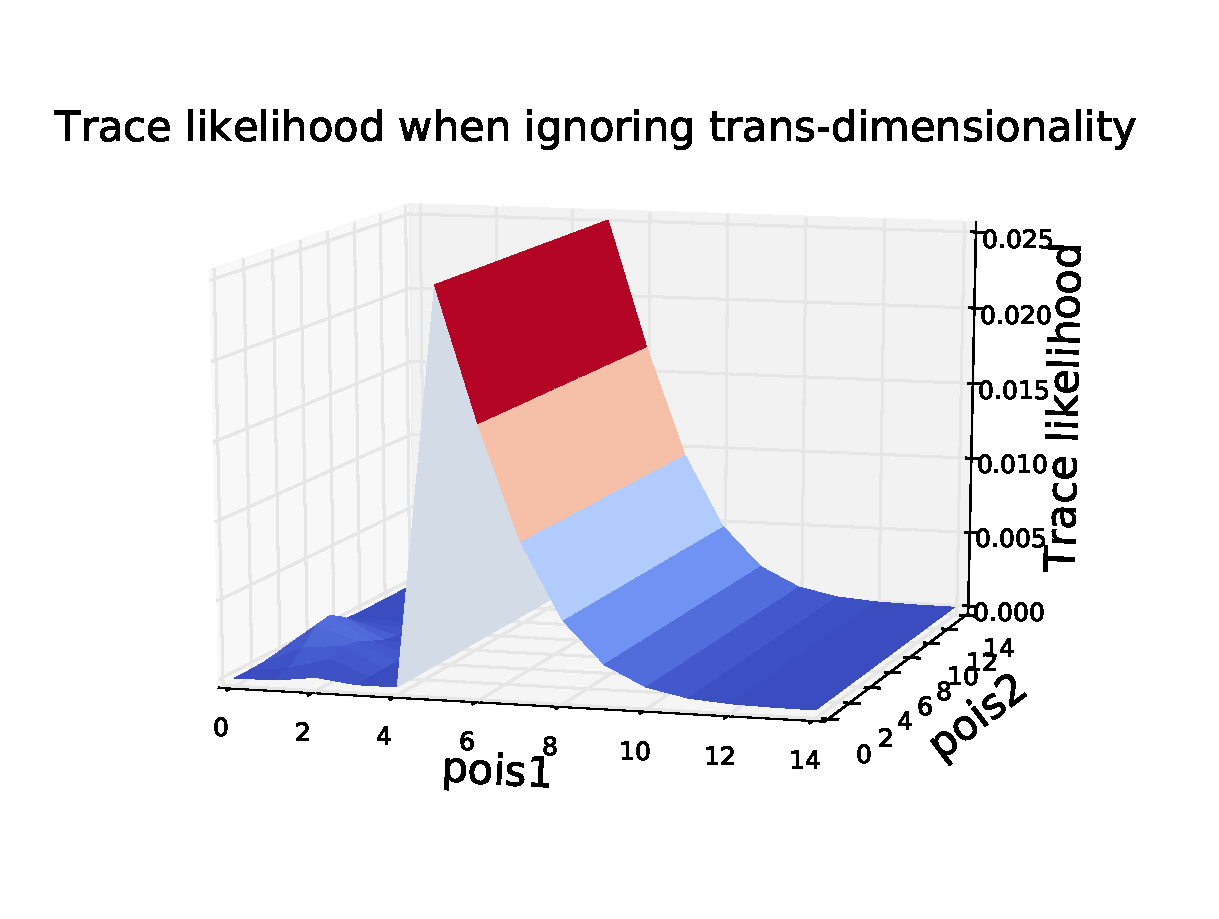
\includegraphics[width=0.8\textwidth]{BranchWrongTraceLik}
    \caption{Space of trace likelihoods implied by naive slice sampling.}
    \label{fig:BranchWrongTraceLik}
\end{figure}

Integrating out the pois2 variable from this likelihood space results in the following implied posterior (see Figrue \ref{fig})

\begin{figure}[H]
    \centering
    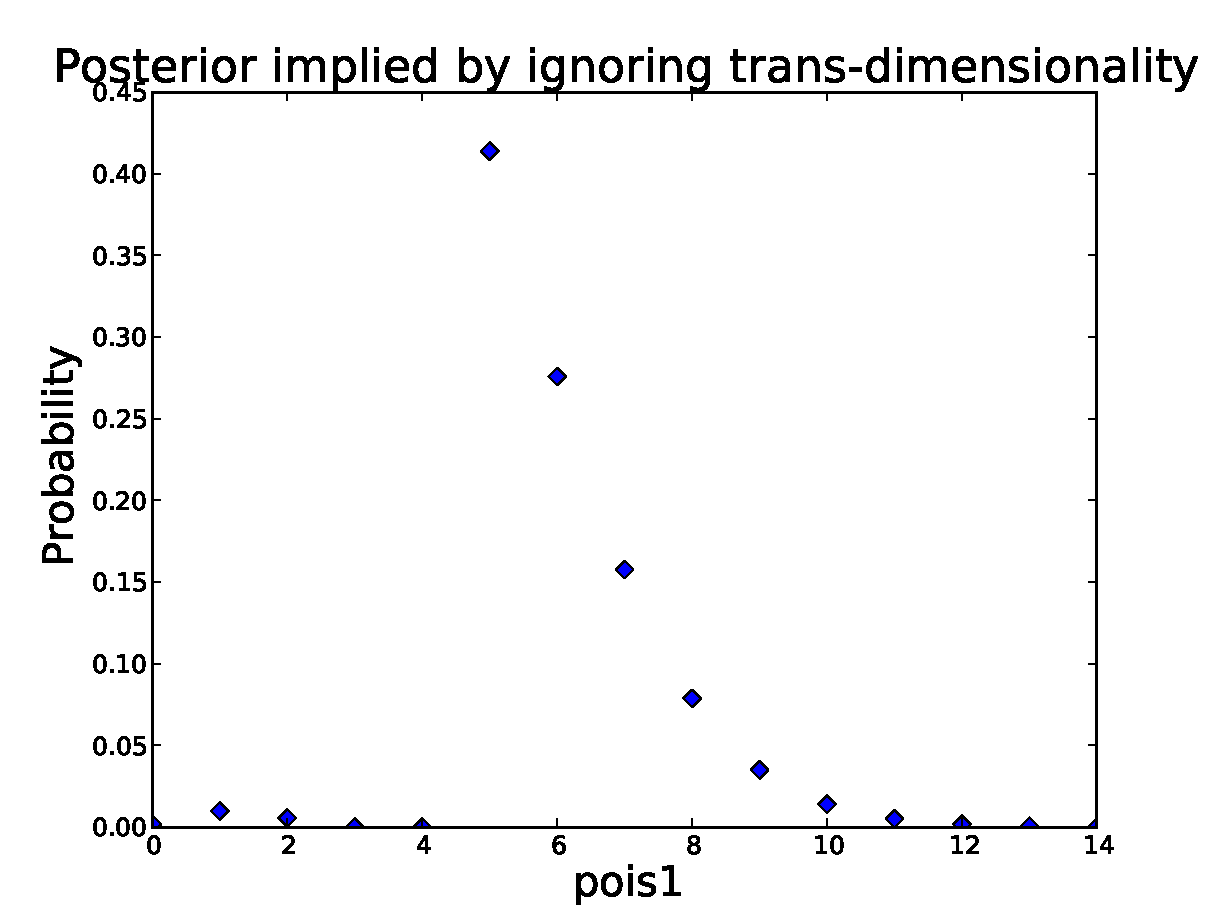
\includegraphics[width=0.8\textwidth]{BranchWrongPost}
    \caption{Branching posterior implied by naive slice sampling.}
    \label{fig:BranchWrongPost}
\end{figure}

This wrong posterior is the one which naive slice sampling will be attempting to infer. \todo{mention buggy metropolis version that also samples from this}

Next we'll look at one simple attempt to correct for trans-dimensional jumps, by thinking in terms of fresh and stale likelihoods, as in the metropolis acceptance ratio.

Specifically, when comparing a trace log-likelihood against the slice's sampled he1ight, we won't simply consider the log likelihood (ll), but instead ll + llStale - llFresh.
This means that when we are considering a jump to a lower dimensional space the log-likelihood of the lower dimensional space will be decreased by llStale (i.e. the likelihoods of the variables which are not part of this space). Conversely, when considering a move to a higher dimensional space, the log-likelihood of the higher-dimensional trace will be discounted by llFresh (so only the likelihood of the subset of variables that are also part of the current, lower-dimensional, space count).

This simple correction seems to give correct results on the continuous NormalMean3 trans-dimensional model explored above (see Figure \ref{fig})

\begin{figure}[H]
    \centering
    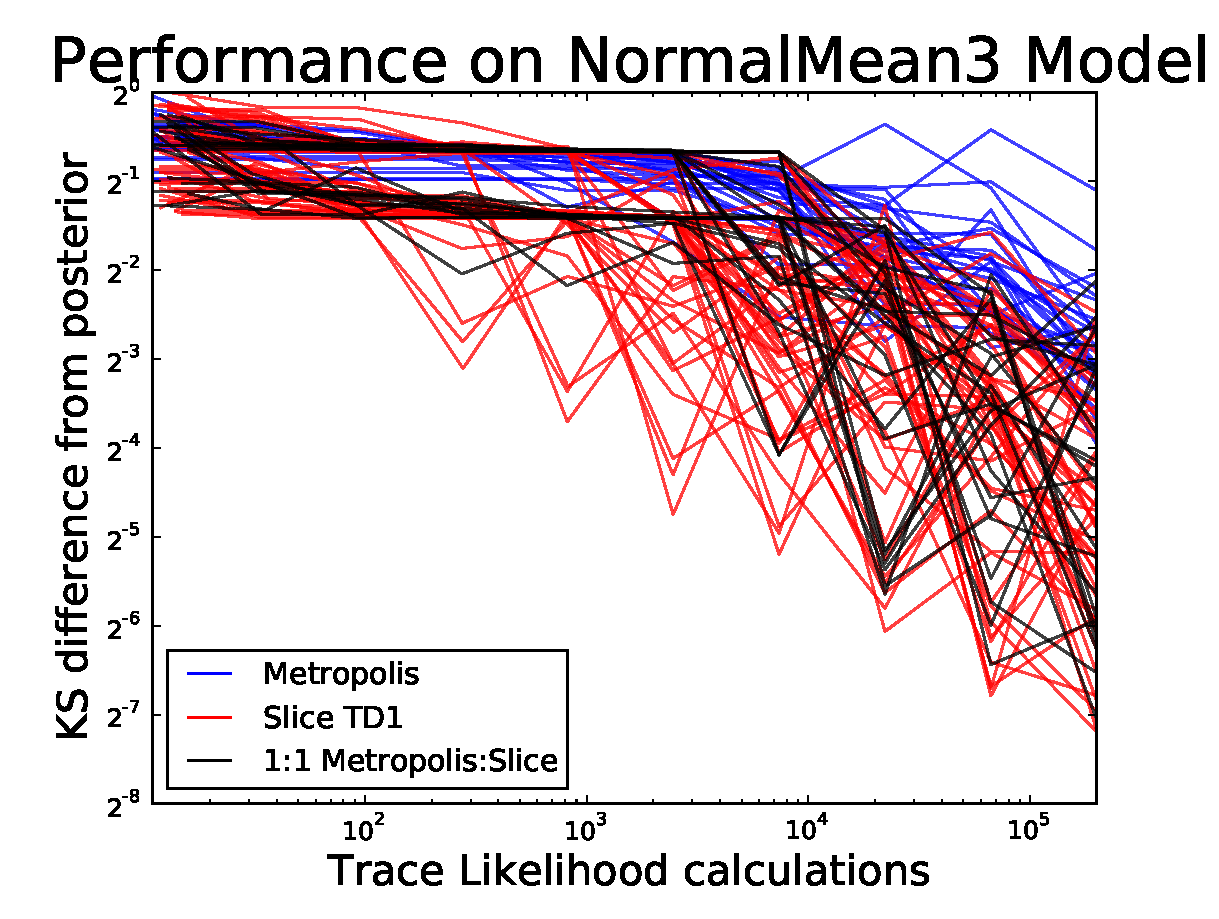
\includegraphics[width=0.8\textwidth]{Normal4TDRuns}
    \caption{Runs generated by metropolis, a 1:1 mixtures of metropolis and slice and the corrected slice on the NormalMean3 model.}
    \label{fig:Normal4TDRuns}
\end{figure}

\begin{figure}[H]
    \centering
    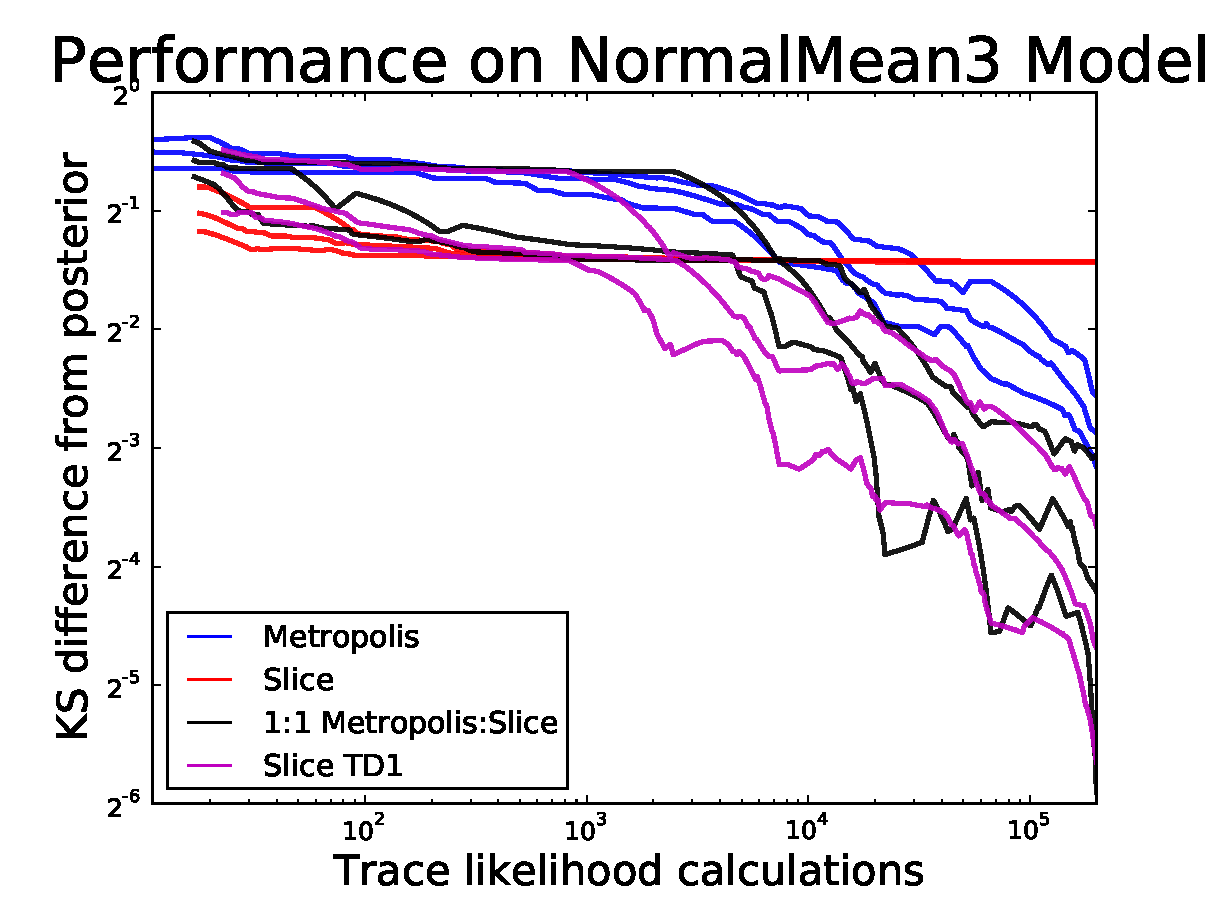
\includegraphics[width=0.8\textwidth]{Normal4TDQuarts}
    \caption{Quartiles of the euns generated by metropolis, a 1:1 mixtures of metropolis and slice, the corrected slice and the naive slice algorithms on the NormalMean3 model.}
    \label{fig:Normal4TDQuarts}
\end{figure}


However, the specification appears to be wrong since it does not converge to the correct distribution on the Branching model (see Figure \ref{fig}). Somewhat interestingly, it does seem to converge to a wrong value that's somewhat closer to the true posterior than the naive slice sampling does.

\begin{figure}[H]
    \centering
    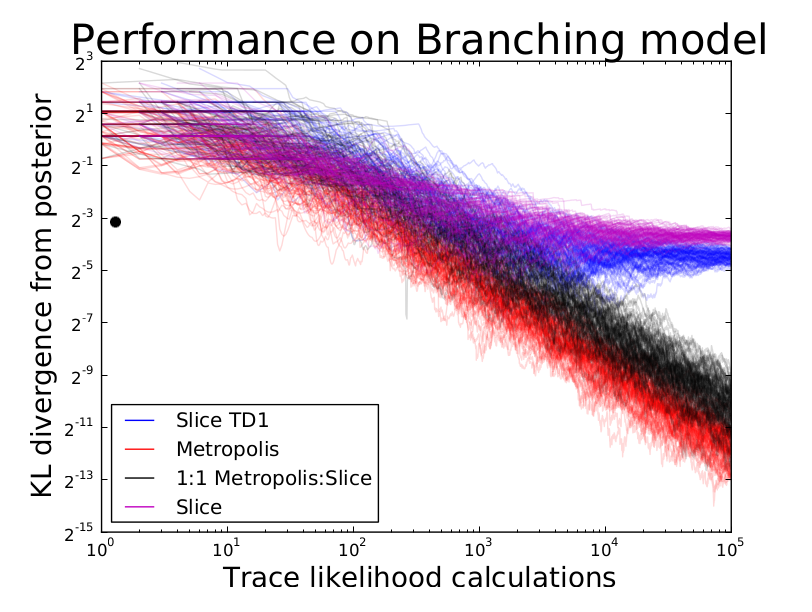
\includegraphics[width=0.8\textwidth]{BranchTDRuns}
    \caption{Runs generated by metropolis, a 1:1 mixtures of metropolis and slice, the corrected slice and the naive slice algorithms on the Branching model.}
    \label{fig:BranchTDRuns}
\end{figure}

\begin{figure}[H]
    \centering
    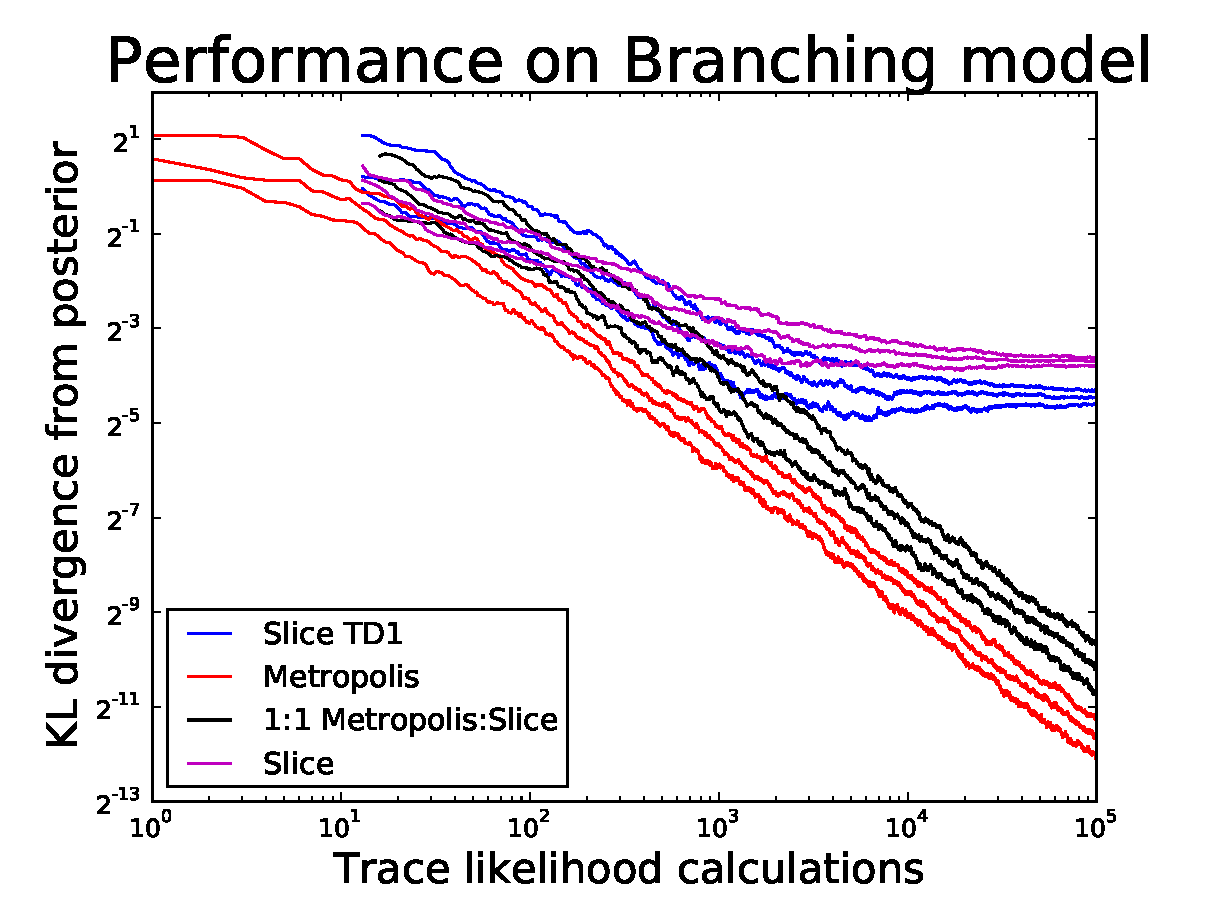
\includegraphics[width=0.8\textwidth]{BranchTDQuarts}
    \caption{Quartiles of the runs generated by metropolis, a 1:1 mixtures of metropolis and slice, the corrected slice and the naive slice algorithms on the Branching model.}
    \label{fig:BranchTDQuarts}
\end{figure}

\section{Quasi-Monte Carlo}
Another possible improvement on naive MC is, instead of sampling randomly from the unit interval, to instead make use of a low-discrepancy sequence that will tend to cover the interval faster.

A simple sequence we can use in the 1-dimensional case is the Van der Corput sequence.
We test the performance of this sequence by considering time to mode of neighbourhood for a interval of size 100, neighbourhood of size 1 and modes in the range $[0.5, 1.5, \ldots 99.5]$
Naive metropolis will find this neighbourhood, on average in 100 steps. Using the Van der Corput sequence reduces this to 56 samples. 

The slice sampling technique explored above, however,  managed reductions to 10 and 20 steps respectively (depending on the likelihood function). Therefore I choose to focus on developing the slice sampling technique rather than further investigation Quasi-Monte Carlo methods.


